\documentclass{article}
\usepackage{fullpage}
\usepackage{amsmath,amssymb,amsthm,bm,bbm,enumerate,mathtools}
\usepackage[hidelinks]{hyperref}
\usepackage{natbib}
\usepackage{xcolor}
\usepackage{graphics}

\newcommand{\E}{\mathbb{E}}
\renewcommand{\P}{\mathbb{P}}
\newcommand{\R}{\mathbb{R}}
\newcommand{\mL}{\mathcal{L}}
\newcommand{\ip}[2]{\left\langle #1, #2 \right\rangle}
\newcommand{\ie}{\textit{i.e.,}\,}
\newcommand{\eg}{\textit{e.g.,}\,}
\newcommand{\nb}{\textit{n.b.,}\, }
\newcommand{\defn}{:=}
\newcommand{\var}{\mathop{\mbox{Var}}}
\newcommand{\cov}{\mathop{\mbox{Cov}}}

\newcommand{\iid}{\overset{i.i.d}{\sim}}
\newcommand{\1}{\mathbbm{1}}
\newcommand{\Oh}{{\mathcal O}}

\newcommand{\comment}[1]{{\color{blue} \it #1}}

\DeclareMathOperator*{\Log}{Log}
\DeclareMathOperator*{\Cauchy}{Cauchy}
\DeclareMathOperator*{\Bernoulli}{Bernoulli}
\DeclareMathOperator*{\sgn}{sgn}
\DeclareMathOperator*{\re}{Re}

\newtheorem{thm}{Theorem}
\newtheorem{lem}{Lemma}
\newtheorem{prop}{Proposition}
\newtheorem{cor}{Corollary}
\theoremstyle{remark} 
	\newtheorem{rem}{Remark}
	\newtheorem{assn}{Assumption}
\theoremstyle{definition} 
	\newtheorem{mydef}{Definition} 
	\newtheorem{exmp}{Example} 
	\newtheorem{cond}{Condition}
	\newtheorem{conj}{Conjecture}

\newif\ifsubmission
\submissiontrue
% \submissionfalse
\ifsubmission
    % % stuff for submission
    \usepackage{lineno}
    % allow line numbers around math environments
    % from https://tex.stackexchange.com/questions/43648/why-doesnt-lineno-number-a-paragraph-when-it-is-followed-by-an-align-equation
        \newcommand*\patchAmsMathEnvironmentForLineno[1]{%
          \expandafter\let\csname old#1\expandafter\endcsname\csname #1\endcsname
          \expandafter\let\csname oldend#1\expandafter\endcsname\csname end#1\endcsname
          \renewenvironment{#1}%
             {\linenomath\csname old#1\endcsname}%
             {\csname oldend#1\endcsname\endlinenomath}}% 
        \newcommand*\patchBothAmsMathEnvironmentsForLineno[1]{%
          \patchAmsMathEnvironmentForLineno{#1}%
          \patchAmsMathEnvironmentForLineno{#1*}}%
        \AtBeginDocument{%
        \patchBothAmsMathEnvironmentsForLineno{equation}%
        \patchBothAmsMathEnvironmentsForLineno{align}%
        \patchBothAmsMathEnvironmentsForLineno{flalign}%
        \patchBothAmsMathEnvironmentsForLineno{alignat}%
        \patchBothAmsMathEnvironmentsForLineno{gather}%
        \patchBothAmsMathEnvironmentsForLineno{multline}%
        }
\else
    % for the nice version
\fi

% Responses to reviews
\usepackage{lineno, hyperref}
% \usepackage[hypertexnames=false]{hyperref}   % not working correctly
% \usepackage{latexml}

\linenumbers


%%%%%  PUT THIS IN HEADER OF FILE
% % Responses to reviews:
% \usepackage{lineno, hyperref}
% \usepackage[hypertexnames=false]{hyperref}   % not working correctly
% \usepackage{latexml}

\linenumbers


%%%%%  PUT THIS IN HEADER OF FILE
% % Responses to reviews:
% \usepackage{lineno, hyperref}
% \usepackage[hypertexnames=false]{hyperref}   % not working correctly
% \usepackage{latexml}

\linenumbers


%%%%%  PUT THIS IN HEADER OF FILE
% % Responses to reviews:
% \input{review-response-commands}
% % set this to show line numbers and include responses to reviews or not
% \newif\ifreviewresponses
% \reviewresponsestrue  % include them
% % \reviewresponsesfalse  % don't include them
% \newcommand{\responsefile}{pbio-reviews-19sept12-responses.tex}  % name of the review reponses file

% counters for reviewer points
%% instead do reviewer labels
% \newcounter{reviewer}
% \setcounter{reviewer}{0}
\newcommand{\thereviewer}{}
\newcounter{point}
\setcounter{point}{0}

% pass in to \reviewersection the label for this reviewer (i.e. \reviewersection{1} or \reviewersection{AE})
\newcommand{\reviewersection}[1]{\renewcommand{\thereviewer}{#1}
                  \setcounter{point}{0}
                  \section*{Reviewer \thereviewer:}}
% drawing from from http://tex.stackexchange.com/questions/2317/latex-style-or-macro-for-detailed-response-to-referee-report
%% arguments to \point are (name of the point, optional) and (content)
\newenvironment{point}[1]
        { \refstepcounter{point} \bigskip \hrule \medskip \noindent 
                \slshape {\fontseries{b}\selectfont (\thereviewer.\thepoint) #1} }
        { }
\newcommand{\reply}{\normalfont \medskip \noindent \textbf{Reply}:\ }   

% use this command in the text where a change addressing a reviewer point has occurred
% e.g. \revpoint{1}{3} for reviewer 1, point 3
\newcommand{\revpoint}[2]{\hypertarget{llineno:rev#1:#2}{\linelabel{rr:rev#1:#2}}}
% and this one to refer to such a location, e.g. \revreffull{1}{3}
\newcommand{\revreffull}[2]{{(p.\ \hyperlink{llineno:rev#1:#2}{\pageref{rr:rev#1:#2}, l.\ \lineref{rr:rev#1:#2}})}}
% but this version fills in reviewer and point automatically if called in the appropriate part of the reviews
\newcommand{\revref}{\revreffull{\thereviewer}{\thepoint}}
% NOTE: should call \revref{} with empty brackets after to get a space afterwards if desired: http://tex.stackexchange.com/questions/31091/space-after-latex-commands

% or, this one to refer to a named linelabel
% e.g. if in the text there is a \llabel{approx_eqn_point}
% refer to it with \llname{approx_eqn_point}
\newcommand{\llabel}[1]{\hypertarget{ll:#1}{\linelabel{#1}}}
\newcommand{\llname}[1]{{(p.\ \hyperlink{ll:#1}{\pageref{#1}, l.\ \lineref{#1}})}}

% put \includereviews() where the reviews are to appear (at the end?)
\newcommand{\includereviews}{
    \ifreviewresponses
    \clearpage
    \setcounter{page}{1}
    \setcounter{section}{0}
    \setcounter{subsection}{0}
    \nolinenumbers
    % \begin{center}
    %   {\LARGE \bf Response to Reviews}
    % \end{center}
    \input{\responsefile}
    \fi
}

% Useful shortcuts ;) that demonstrate how to use the macros.
\newcommand{\rollover}{ \reply{The reviewer makes an excellent point that we have missed out entirely.  We have made all the changes suggested, down to the minutiae \revref.} }
\newcommand{\playdead}{ \reply{The reviewer makes an excellent point.  We have made an utterly trivial change {\revref} that we think deals entirely with the concern raised.} }
                                                                                                         
% from http://tex.stackexchange.com/questions/43648/why-doesnt-lineno-number-a-paragraph-when-it-is-followed-by-an-align-equation/55297#55297
\ifcsname{patchAmsMathEnvironmentForLineno}\endcsname
    \newcommand*\patchAmsMathEnvironmentForLineno[1]{%                                                       
      \expandafter\let\csname old#1\expandafter\endcsname\csname #1\endcsname                                
      \expandafter\let\csname oldend#1\expandafter\endcsname\csname end#1\endcsname                          
      \renewenvironment{#1}%                                                                                 
         {\linenomath\csname old#1\endcsname}%                                                               
         {\csname oldend#1\endcsname\endlinenomath}}%                                                        
    \newcommand*\patchBothAmsMathEnvironmentsForLineno[1]{%                                                  
      \patchAmsMathEnvironmentForLineno{#1}%                                                                 
      \patchAmsMathEnvironmentForLineno{#1*}}%                                                               
    \AtBeginDocument{%                                                                                       
    \patchBothAmsMathEnvironmentsForLineno{equation}%                                                        
    \patchBothAmsMathEnvironmentsForLineno{align}%                                                           
    \patchBothAmsMathEnvironmentsForLineno{flalign}%                                                         
    \patchBothAmsMathEnvironmentsForLineno{alignat}%                                                         
    \patchBothAmsMathEnvironmentsForLineno{gather}%                                                          
    \patchBothAmsMathEnvironmentsForLineno{multline}%                                                        
\fi

% % set this to show line numbers and include responses to reviews or not
% \newif\ifreviewresponses
% \reviewresponsestrue  % include them
% % \reviewresponsesfalse  % don't include them
% \newcommand{\responsefile}{pbio-reviews-19sept12-responses.tex}  % name of the review reponses file

% counters for reviewer points
%% instead do reviewer labels
% \newcounter{reviewer}
% \setcounter{reviewer}{0}
\newcommand{\thereviewer}{}
\newcounter{point}
\setcounter{point}{0}

% pass in to \reviewersection the label for this reviewer (i.e. \reviewersection{1} or \reviewersection{AE})
\newcommand{\reviewersection}[1]{\renewcommand{\thereviewer}{#1}
                  \setcounter{point}{0}
                  \section*{Reviewer \thereviewer:}}
% drawing from from http://tex.stackexchange.com/questions/2317/latex-style-or-macro-for-detailed-response-to-referee-report
%% arguments to \point are (name of the point, optional) and (content)
\newenvironment{point}[1]
        { \refstepcounter{point} \bigskip \hrule \medskip \noindent 
                \slshape {\fontseries{b}\selectfont (\thereviewer.\thepoint) #1} }
        { }
\newcommand{\reply}{\normalfont \medskip \noindent \textbf{Reply}:\ }   

% use this command in the text where a change addressing a reviewer point has occurred
% e.g. \revpoint{1}{3} for reviewer 1, point 3
\newcommand{\revpoint}[2]{\hypertarget{llineno:rev#1:#2}{\linelabel{rr:rev#1:#2}}}
% and this one to refer to such a location, e.g. \revreffull{1}{3}
\newcommand{\revreffull}[2]{{(p.\ \hyperlink{llineno:rev#1:#2}{\pageref{rr:rev#1:#2}, l.\ \lineref{rr:rev#1:#2}})}}
% but this version fills in reviewer and point automatically if called in the appropriate part of the reviews
\newcommand{\revref}{\revreffull{\thereviewer}{\thepoint}}
% NOTE: should call \revref{} with empty brackets after to get a space afterwards if desired: http://tex.stackexchange.com/questions/31091/space-after-latex-commands

% or, this one to refer to a named linelabel
% e.g. if in the text there is a \llabel{approx_eqn_point}
% refer to it with \llname{approx_eqn_point}
\newcommand{\llabel}[1]{\hypertarget{ll:#1}{\linelabel{#1}}}
\newcommand{\llname}[1]{{(p.\ \hyperlink{ll:#1}{\pageref{#1}, l.\ \lineref{#1}})}}

% put \includereviews() where the reviews are to appear (at the end?)
\newcommand{\includereviews}{
    \ifreviewresponses
    \clearpage
    \setcounter{page}{1}
    \setcounter{section}{0}
    \setcounter{subsection}{0}
    \nolinenumbers
    % \begin{center}
    %   {\LARGE \bf Response to Reviews}
    % \end{center}
    \input{\responsefile}
    \fi
}

% Useful shortcuts ;) that demonstrate how to use the macros.
\newcommand{\rollover}{ \reply{The reviewer makes an excellent point that we have missed out entirely.  We have made all the changes suggested, down to the minutiae \revref.} }
\newcommand{\playdead}{ \reply{The reviewer makes an excellent point.  We have made an utterly trivial change {\revref} that we think deals entirely with the concern raised.} }
                                                                                                         
% from http://tex.stackexchange.com/questions/43648/why-doesnt-lineno-number-a-paragraph-when-it-is-followed-by-an-align-equation/55297#55297
\ifcsname{patchAmsMathEnvironmentForLineno}\endcsname
    \newcommand*\patchAmsMathEnvironmentForLineno[1]{%                                                       
      \expandafter\let\csname old#1\expandafter\endcsname\csname #1\endcsname                                
      \expandafter\let\csname oldend#1\expandafter\endcsname\csname end#1\endcsname                          
      \renewenvironment{#1}%                                                                                 
         {\linenomath\csname old#1\endcsname}%                                                               
         {\csname oldend#1\endcsname\endlinenomath}}%                                                        
    \newcommand*\patchBothAmsMathEnvironmentsForLineno[1]{%                                                  
      \patchAmsMathEnvironmentForLineno{#1}%                                                                 
      \patchAmsMathEnvironmentForLineno{#1*}}%                                                               
    \AtBeginDocument{%                                                                                       
    \patchBothAmsMathEnvironmentsForLineno{equation}%                                                        
    \patchBothAmsMathEnvironmentsForLineno{align}%                                                           
    \patchBothAmsMathEnvironmentsForLineno{flalign}%                                                         
    \patchBothAmsMathEnvironmentsForLineno{alignat}%                                                         
    \patchBothAmsMathEnvironmentsForLineno{gather}%                                                          
    \patchBothAmsMathEnvironmentsForLineno{multline}%                                                        
\fi

% % set this to show line numbers and include responses to reviews or not
% \newif\ifreviewresponses
% \reviewresponsestrue  % include them
% % \reviewresponsesfalse  % don't include them
% \newcommand{\responsefile}{pbio-reviews-19sept12-responses.tex}  % name of the review reponses file

% counters for reviewer points
%% instead do reviewer labels
% \newcounter{reviewer}
% \setcounter{reviewer}{0}
\newcommand{\thereviewer}{}
\newcounter{point}
\setcounter{point}{0}

% pass in to \reviewersection the label for this reviewer (i.e. \reviewersection{1} or \reviewersection{AE})
\newcommand{\reviewersection}[1]{\renewcommand{\thereviewer}{#1}
                  \setcounter{point}{0}
                  \section*{Reviewer \thereviewer:}}
% drawing from from http://tex.stackexchange.com/questions/2317/latex-style-or-macro-for-detailed-response-to-referee-report
%% arguments to \point are (name of the point, optional) and (content)
\newenvironment{point}[1]
        { \refstepcounter{point} \bigskip \hrule \medskip \noindent 
                \slshape {\fontseries{b}\selectfont (\thereviewer.\thepoint) #1} }
        { }
\newcommand{\reply}{\normalfont \medskip \noindent \textbf{Reply}:\ }   

% use this command in the text where a change addressing a reviewer point has occurred
% e.g. \revpoint{1}{3} for reviewer 1, point 3
\newcommand{\revpoint}[2]{\hypertarget{llineno:rev#1:#2}{\linelabel{rr:rev#1:#2}}}
% and this one to refer to such a location, e.g. \revreffull{1}{3}
\newcommand{\revreffull}[2]{{(p.\ \hyperlink{llineno:rev#1:#2}{\pageref{rr:rev#1:#2}, l.\ \lineref{rr:rev#1:#2}})}}
% but this version fills in reviewer and point automatically if called in the appropriate part of the reviews
\newcommand{\revref}{\revreffull{\thereviewer}{\thepoint}}
% NOTE: should call \revref{} with empty brackets after to get a space afterwards if desired: http://tex.stackexchange.com/questions/31091/space-after-latex-commands

% or, this one to refer to a named linelabel
% e.g. if in the text there is a \llabel{approx_eqn_point}
% refer to it with \llname{approx_eqn_point}
\newcommand{\llabel}[1]{\hypertarget{ll:#1}{\linelabel{#1}}}
\newcommand{\llname}[1]{{(p.\ \hyperlink{ll:#1}{\pageref{#1}, l.\ \lineref{#1}})}}

% put \includereviews() where the reviews are to appear (at the end?)
\newcommand{\includereviews}{
    \ifreviewresponses
    \clearpage
    \setcounter{page}{1}
    \setcounter{section}{0}
    \setcounter{subsection}{0}
    \nolinenumbers
    % \begin{center}
    %   {\LARGE \bf Response to Reviews}
    % \end{center}
    \input{\responsefile}
    \fi
}

% Useful shortcuts ;) that demonstrate how to use the macros.
\newcommand{\rollover}{ \reply{The reviewer makes an excellent point that we have missed out entirely.  We have made all the changes suggested, down to the minutiae \revref.} }
\newcommand{\playdead}{ \reply{The reviewer makes an excellent point.  We have made an utterly trivial change {\revref} that we think deals entirely with the concern raised.} }
                                                                                                         
% from http://tex.stackexchange.com/questions/43648/why-doesnt-lineno-number-a-paragraph-when-it-is-followed-by-an-align-equation/55297#55297
\ifcsname{patchAmsMathEnvironmentForLineno}\endcsname
    \newcommand*\patchAmsMathEnvironmentForLineno[1]{%                                                       
      \expandafter\let\csname old#1\expandafter\endcsname\csname #1\endcsname                                
      \expandafter\let\csname oldend#1\expandafter\endcsname\csname end#1\endcsname                          
      \renewenvironment{#1}%                                                                                 
         {\linenomath\csname old#1\endcsname}%                                                               
         {\csname oldend#1\endcsname\endlinenomath}}%                                                        
    \newcommand*\patchBothAmsMathEnvironmentsForLineno[1]{%                                                  
      \patchAmsMathEnvironmentForLineno{#1}%                                                                 
      \patchAmsMathEnvironmentForLineno{#1*}}%                                                               
    \AtBeginDocument{%                                                                                       
    \patchBothAmsMathEnvironmentsForLineno{equation}%                                                        
    \patchBothAmsMathEnvironmentsForLineno{align}%                                                           
    \patchBothAmsMathEnvironmentsForLineno{flalign}%                                                         
    \patchBothAmsMathEnvironmentsForLineno{alignat}%                                                         
    \patchBothAmsMathEnvironmentsForLineno{gather}%                                                          
    \patchBothAmsMathEnvironmentsForLineno{multline}%                                                        
\fi

% set this to show line numbers and include responses to reviews or not
\newif\ifreviewresponses
\reviewresponsestrue  % include them
% \reviewresponsesfalse  % don't include them
\newcommand{\responsefile}{review-responses}  % name of the review responses file


\begin{document}

% Intro:
%  - the infinitesimal model is useful because it is a "trait-only" model: it allows for predictions and modeling without knowing the underlying genetics.
%  - Its key properties are: (a) independence of seg noise, and (b) Gaussian-ness.
%  - It is basically a CLT, and in particular, (b) derives from a the CLT deriving from similar effect sizes.
%  - Motivating Q: there are other CLTs; can we generalize (b) to non-Gaussian effects, while keeping independence of seg variation?
% 
% Data motivation:
%  First, to see if this is worth asking we look at some data
%  ... and find that yeah, maybe effect sizes don't fall into the Gaussian domain of attraction.
% 
% First answer to the motivating question:  "No"
% Non-Gaussian effects (sometimes) imply nonindependence of transmission noise:
%   In at least some cases, natural non-gaussian models produce nonindependence:
%   1. all loci are uniformly small except there's one big one
%   2. loci are Cauchy
%   3. (is there a simple statement we can make more generally?)
% 
% Second answer, weaker but also "no":
%  - Observation: Let A and B be the contributions to parent phenotype, with A inherited by the offspring and B not. If A and B are independent, and seg noise is independent of parent phenotype, then A and B are Gaussian.
%  - When would A and B be asymptotically independent? One case is the rare-mutation limit that obtains a "thinned Poisson process" limit for A and B (I think: if all allele frequencies are at frequency O(1/M)?)
%  - (I have other thoughts to be sorted out here)
%  - Open Q (maybe?): is there any non-Gaussian model where transmission noise is independent of parental traits?
% 
% Simulations: let's see how this stuff works in practice
%  - neutral simulations
%  - also, stabilizing selection with theoretical motivation for form of stabilizing selection
%  - plot: (A) trait mean over time and trait distribution at the end
%  - plot: (B) (distrn of seg noise), (seg noise vs midparent), and (Radon-Nicodym deriv of conditional seg noise for a few values of midparent)
% 
% If we remove 'big loci' is what's left the infinitesimal model?
%  - people do this in practice (animal breeding papers)
%  - theory:  form of limiting conditional distribution
%  - theory: something about independence  (?? if we get there ??)
%  - plots (A) & (B) above from simulation, but for only small effects


\title{\large{\bf
    Large effects and the infinitesimal model
}}

\author{ \begin{small}
    Todd L. Parsons\footnote{LPSM, Sorbonne Universit\'e, CNRS UMR 8001, Paris, France, 75005}
    ~\&~
    Peter L. Ralph\footnote{Institute of Ecology \& Evolution, University of Oregon, Eugene, OR, USA, 97405}
\end{small}}

\date{\today}
\maketitle

\begin{abstract}
    The infinitesimal model of quantitative genetics
    relies on the Central Limit Theorem to stipulate that
    under additive models of quantitative traits
    determined by many loci having similar effect size,
    the difference between an offspring's genetic trait component
    and the average of their two parents' genetic trait components
    is Normally distributed and independent of the parents' values.
    Here, we investigate how the assumption of similar effect sizes
    affects the model:
    in particular, if the tail of the effect size distribution is polynomial
    with exponent $\alpha < 2$, then sums of effects
    should be well-approximated by a ``stable distribution'',
    and find tail exponents between 1 and 2 in 
    effect sizes estimated by genome-wide association studies
    of many human disease-related traits.
    We show that the independence of offspring trait deviations from parental averages
    in many cases implies a Gaussian distribution,
    suggesting that non-Gaussian models of trait evolution must explicitly
    track the underlying genetics, at least for loci of large effect.
    We also characterize possible limiting trait distributions
    of the infinitesimal model with infinitely divisible noise distributions,
    and compare our results to simulations.
\end{abstract}

\comment{ADD TO DISCUSSION, WHICH IS SHORT:
    Make the point that another way to think about distibutions with non-finite variance
    is that there's only a finite number of alleles above any fixed value;
    and also the variance in any finite population will be finite.
    (see reviewer comment, ``all the empirical trait distributions they find have mean and variance'')
    Also discuss comparison to fat-tailed dispersal:
    the question is, what distribution gives us a better model?
    For dispersal, a fat-tailed distribution has in practice finite variance
    but is a better model in that it describes noisiness better;
    here, the analogy is something about polygenicity and noisiness of the process of adaptation.
    If we're modeling non-polygenic (oligogenic) traits then
    why stable as opposed to some other arbitrary distribution?
    Well, the distribution of per-allele effect sizes might not be stable, but CLT tells us that maybe
    stable gives a good approx to the process (as in Gaussian case).
}

%%%%%%%%%%%%%%%%%%%%%%
\section{Introduction}

Much of the work to 
understand the evolution of quantitative traits in sexual species
has focused on models in quantitative genetics
that describe evolution of trait values without explicitly representing underlying genetic variation,
but in a manner deriving from our understanding of how genetic variation works in practice.
Such models are therefore
interestingly intermediate between mechanistic models of genetics and purely phenomenological.
% The action of natural selection on genetic variants in the absence of genetic variation is relatively well-understood (cite ewens),
% but tractable mathematical models of evolution for recombining species are elusive,
% at least with some results of when the model might be a good description of reality.
% For instance, a great deal of conceptual understanding and even quantitative predictions
% have been made assuming that the distribution of trait values in a population is Gaussian (cite Lande etcetera)
% despite the absence of a plausible model that would make this true (cite turelli and barton).
One concrete model of heritable trait evolution is the \emph{infinitesimal model},
which assumes a simple, explicit form for how the genetic component of offsprings' traits are determined by their parents:
they are Normally distributed, with the mean for each offspring equal to the average of the parents' values,
and a covariance independent of the parental trait values (but that depends on how they are related).
\citet{barton2017infinitesimal} give a history of the model
and a formal proof of conditions under which this would be a good approximation to reality,
which they extended to include dominance in \citet{barton2022infinitesimal}.

As suggested by its name,
under the infinitesimal model the effects of any given genetic variant on the trait
is small (indeed, vanishing),
and selection-driven trait shifts are mediated by small changes in frequencies of many alleles of small effect.
However, empirical understanding of the genetic basis of trait variation in real-world species
often finds a significant portion of heritable variation explained by variants at only a few loci.
There are many possible explanations for this observation,
including selection or publication bias,
filters for larger-effect variants due to spatially varying selection
\citep{barton1987establishment,yeaman2011establishment,yeaman2011genetic},
and/or grouping together of concordant alleles by linkage or inversions
\citep{kirkpatrick2006chromosome}.
However,
it seems clear that in at least those cases where we understand the underlying molecular mechanisms,
mutations of large effect can be important in practice.
% \citep[e.g.,][]{cyclodiene-resistance,hoekstra2006genetics}.
The consensus in the field seems to be that traits exist on a spectrum between monogenic and polygenic,
and that many -- if not most -- lie in the intermediate region,
where heritable trait variation is due both to segregating large- and small-effect variants.
Indeed, some sensible verbal models of the biological mechanisms by which a genetic change
comes to have an effect on an organism's trait
describe a hierarchy or range of ``proximities'' to the trait,
by which changes to more ``nearby'' genes have the possibility of causing larger changes in the trait
\citep{kopp2012transcriptional,boyle2017expanded}.
This suggests a mixture model for the effect size distribution:
perhaps a trait is affected by mutations in a number of genomic regions,
and the distribution of effect sizes within each region is Normal, \revpoint{1}{13}
but with a standard deviation that varies with ``proximity'' of that region to the trait
(e.g., regions that are further ``upstream'' have higher standard deviations).
Such mixtures can easily have large proportions of extreme values.

The Gaussian distribution appears thanks to ``the'' Central Limit Theorem,
i.e., the universality of adding up a great many very small and independent things.
However, there is a wider class of Central Limit Theorems,
which describe the distributions of sums of a great many independent and exchangeable things:
the \emph{stable laws} \citep{gnedenko1968limit}.
Roughly speaking, these say that if we add together $n$ independent copies of a random variable $X$
for which $\P\{ X > t \}$ is proportional to $t^{-\alpha}$ for some $0 < \alpha < 2$,
then -- almost regardless of the details -- the result, scaled by $n^{1/\alpha}$,
is well-approximated by a universal form, an $\alpha$-stable distribution
(and the approximation becomes exact, as $n \to \infty$).
Oth the other hand, if $\alpha \ge 2$ then the distribution has finite variance,
and so the sum of $n$, divided by $\sqrt{n}$, converges to a Gaussian distribution.
In such ensembles, single large entries can be important:
concretely, the largest of the $n$ copies will be of order $n^{1/\alpha}$,
so that e.g., for $\alpha=1$ a positive proportion of the sum of $n$ entries will be contributed by a single one.
On the other hand, the largest of $n$ Gaussians is of order $\sqrt{\log n}$. \revpoint{2}{1}

This suggests exploring whether stable distributions might reasonably stand in for the Gaussian
in the infinitesimal model. \revpoint{1}{1}
In this paper, we make preliminary explorations in that direction:
Do the results of \citet{barton2017infinitesimal}
carry over when the distribution of effect sizes falls in the domain of attraction of a stable law?
The immediate answer to this will be ``no'' --
in fact, we will see that independence of offsprings' deviations and midparent values \emph{implies} a Gaussian distribution for the offsprings' deviations, in some sense. \revpoint{1}{2}
This independence is a key reason why the infinitesimal model is tractable,
and so a conclusion is that additive models with non-Gaussian effects may not be well-approximated
by ``trait-only'' models that do not explicitly represent underlying genetic variation.
Having thus shown that ``infinitesimal models with non-Gaussian noise'' is on weak footing as a model of reality,
we then go on to analyze exactly these models.
(As motivation,
we have not shown that such models are \emph{not} good approximations to reality,
and it is interesting and perhaps informative to understand how the noise distribution affects results.)

Stable distributions are by no means new to population biology.
For instance, it is a long-standing question how often the motions of organisms
are better modeled by essentially Brownian random walks or by L\'evy processes \citep{benhamou2007animals}
and a growing literature studies the effects of such power law distributions
on spatial genetic patterns and evolutionary dynamics
\citep[e.g.,][]{paulose2019spatial,smith2023isolation}.
More directly analogous to the problem we study here, \citet{landis2012phylogenetic}
found that an $\alpha$-stable process (with $\alpha \approx 3/2$) fit the evolution of log endocranial volume
on the primate phylogeny
better than a Brownian model.
It is also important to note that
the infinitesimal model implies a Gaussian distribution for the difference between an offspring's trait and their parents' average,
\emph{not} for the entire population.
The question of when the trait distribution in an evolving population
might be modeled as a Gaussian has been discussed extensively
\citep[e.g.,][]{turelli1994genetic,dbarre2015evolution}.

The ways in which genetic variants affect an organisms' trait can be complex,
and interactions between alleles, between loci, and with the environment are often important in practice.
In fact, many traits claimed to be genetically determined \revpoint{1}{14}
in fact only appear heritable through non-genetic means,
e.g., systematic inequalities in resource distribution partitioned by class or race.
% \citep[e.g.,][]{davenport1916hereditary}.
In this paper, we follow the literature in working with the relatively simple purely additive case
of a trait that can be decomposed into a sum across loci of the contributions of the alleles from each locus,
even omitting an independent effect of ``the environment''.
However, we emphasize that such models should not always be the default for understanding biological variation,
especially for human traits.

%%%%%%%%%%%%%%%%%%%%%%
\subsection*{Notation}

We generally follow the notation of \citet{barton2017infinitesimal},
although in a simpler situation,
as we do not consider full pedigrees
but rather only the haploid offspring of a single set of haploid parents
(as produced, for instance, by a round of meiosis in a diploid stage),
and ignore non-genetic contributions to the trait;
so, below we say ``trait'' to mean ``genetic contribution to the trait''.

Suppose that the focal individual's trait is
$$
    Z_M = \sum_{\ell=1}^M \eta_\ell / M^{1/\alpha},
$$
where $\eta_\ell$ is the contribution of the allele carried at the $\ell^\text{th}$ locus,
and $M$ is the number of loci. \revpoint{2}{2}
The effects of the alleles carried by the two parents
are $\eta_\ell^{[1]}$ and $\eta_\ell^{[2]}$, respectively,
and their traits are
$Z_M^{[1]} = \sum_\ell \eta_\ell^{[1]} / M^{1/\alpha}$ and
$Z_M^{[2]} = \sum_\ell \eta_\ell^{[2]} / M^{1/\alpha}$.
We assume the loci are unlinked and inheritance is fair, so
letting $X_\ell$ be a family of Bernoulli(1/2) random variables that are independent of everything else,
$$
    \eta_\ell = X_\ell \eta_\ell^{[1]} + (1 - X_\ell) \eta_\ell^{[2]} .
$$
What we will call the \emph{Mendelian sampling term}
(or occasionally \emph{Mendelian noise}), $R_M$,
is the offspring's trait minus the midparent value, $\bar Z_M$:
\begin{align*}
    \bar Z_M &= \frac{Z_M^{[1]} + Z_M^{[2]}}{2} \\
    R_M &= Z_M - \bar Z_M \\
        &= \sum_{\ell=1}^M
            \frac{
                X_\ell (\eta_\ell^{[1]} - \eta_\ell^{[2]})
                + (1 - X_\ell) (\eta_\ell^{[2]} - \eta_\ell^{[1]})
            }{ 2 } .
\end{align*}
Note in particular that
the contribution of locus $\ell$ to $R_M$ is $\pm |\eta_\ell^{[1]} - \eta_\ell^{[2]}|$.


%%%%%%%%%%%%%%%%%%%%%%
\section{Empirical observations}
    \label{sec:empirical}

It is mathematically intriguing to speculate what effect a power law effect size distribution
for would have on the induced evolutionary dynamics.
But, is there any evidence that non-Gaussian effects are important in practice?
In this paper we focus primarily on the theory,
but first take a brief and imperfect look at what some data have to say on the topic.
To do this, we downloaded the GWAS results provided by~\citet{biobankSNPs}
for 7,221 phenotypes from 361,194 human individuals from the March 2018 release of the UK Biobank.
After filtering (see details below) we were left with 695 binary illness-related phenotypes.
Taken at face value, these provide for each phenotype a set of estimates of the additive effect
of the alternative allele at a set of single nucleotide polymorphisms (SNPs)
on the phenotype relative to the reference allele.
The phenotypes we consider were all binary and coded as 0/1,
so estimates could be thought of as additive adjustments to the risk
(so, effects are \emph{not} on a logit scale).
These estimates were obtained as the coefficient for the SNP in a simple linear model
fit to each phenotype for each SNP,
with the first 20 principal components and all combinations of age, age squared, and inferred sex as covariates;
we considered effects of those SNPs with a reported $p$-value less than $10^{-8}$.
There are a great many possible issues with these data;
however, the results seem consistent across many SNPs and phenotypes,
and we know of no reason that possible methodological artifacts
(e.g., confounding by uncorrected variables)
would specifically affect the decay of the tail of effect sizes.

Since the Mendelian sampling term is a sum of terms of the form
$$
    (X_\ell - 1/2) \eta_\ell^{[1]} + (1/2 - X_\ell) \eta_\ell^{[2]},
$$
where $\eta_\ell^{[i]}$ is the effect of the allele in parent $i$ at locus $\ell$,
the appropriate central limit theorem for the sum is determined by
the tail behavior of $|(X - 1/2) \eta|$,
where $X$ is Bernoulli(1/2) and $\eta$ is the effect
of a uniformly chosen one of the two alleles from a uniformly chosen parent
at a uniformly chosen locus.
Since $|X-1/2| = 1/2$, we'd like to know
if $\P\{|X|>2t\}$ is proportional to $t^{-\alpha}$,
i.e., the value of
$$
    \lim_{t \to \infty} \frac{ - \log \P\{ |X| > 2 t \} }{ \log t } = \alpha ,
$$
if the limit exists.
Let $p_\ell$ be the minor allele frequency at the $\ell^\text{th}$ locus;
since the data we have assigns effect 0 to the major allele,
$\eta_\ell = 0$ with probability $1-p_\ell$.
Therefore, if we have estimated effects for $M$ SNPs
with minor allele frequency $p_\ell$ and effect size $e_\ell$ for the minor allele,
for $1 \le \ell \le M$,
then
$$
    \P\{ |\eta| > 2t \} \approx \frac{1}{M} \sum_{\ell : |e_\ell| > 2t} p_\ell .
$$
Note that the relevant effect size distribution here is weighted by frequency, \revpoint{1}{3}
which is necessary because we're looking at the deviation of a typical offspring from their parents,
and the chance a given allele is carried by a random parent is given by the frequency.
This will make a difference as frequencies and effect sizes are often correlated in practice.
So, to obtain a per-trait estimate of $\alpha$,
we plot $\log \frac{1}{M} \sum_{\ell : |e_\ell| > t} p_\ell$ against $\log t$
for a sequence of values of $t$,
and fit a linear model to the tail.
(To do this,
we take as the ``tail''
all values of $t$ for which the number of SNPs with absolute effect above $t$
is at least 20 and at most 10\% of all SNPs.) \revpoint{2}{3}
Examples are shown in Figure~\ref{fig:example_snps}.

\begin{figure}
    \begin{center}
    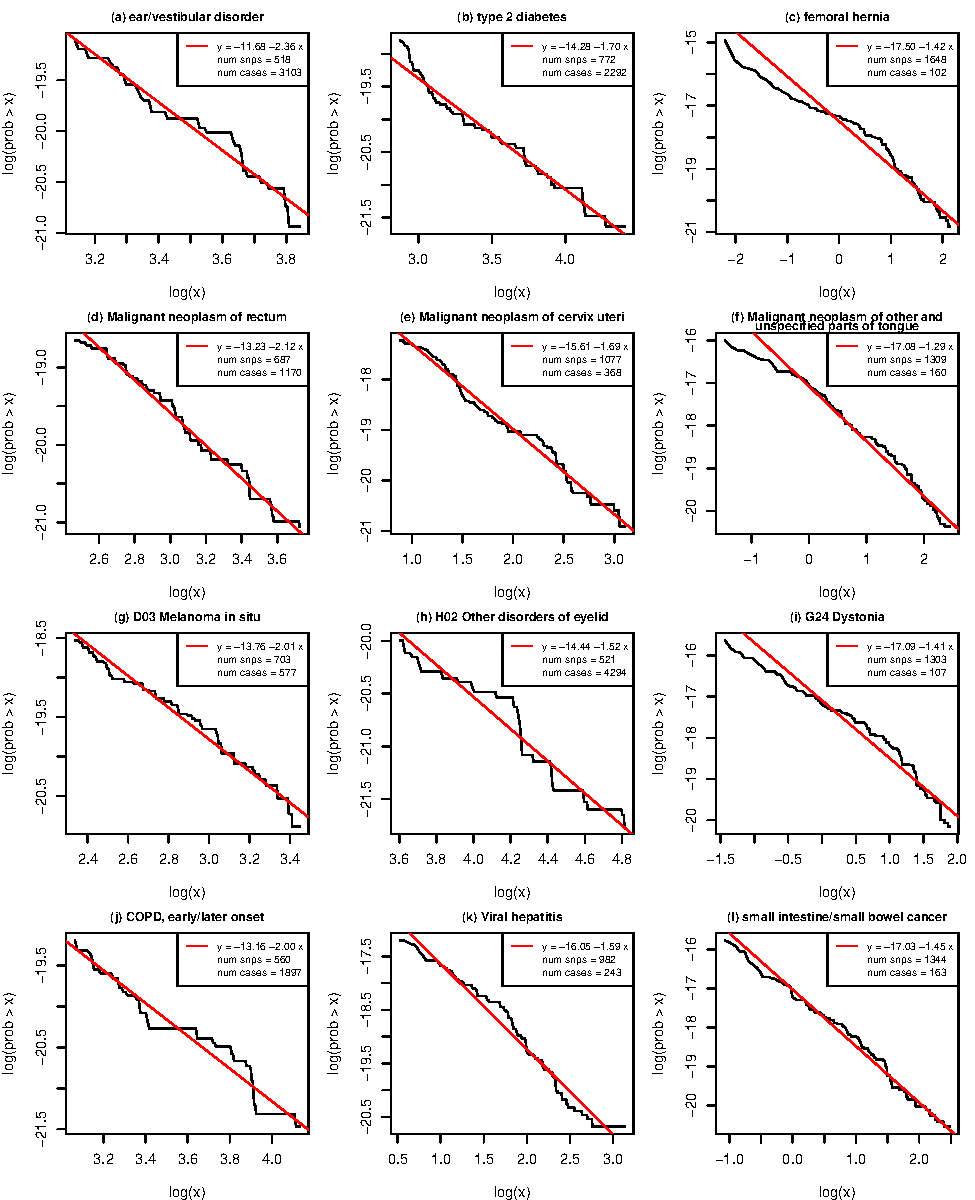
\includegraphics{snp_effects/examples}
    \end{center}
    \caption{
        % TODO: cut this down to just 2 SNPs and move this figure to the supplement; change 'x' to 't' in axis labels.
        Tail distributions of frequency-weighted effects
        for twelve randomly chosen phenotypes.
        In each, for a phenotype with $N$ SNPs,
        effect sizes $e_i$ and frequencies $p_i$,
        the black line shows
        $\log \frac{1}{N} \sum_{i : |e_i| > t} p_i$ (vertical axis)
        against $\log t$ (horizontal axis);
        the red line shows the least-squares linear fit;
        each plot only covers the 10\% largest-effect SNPs.
        Legends show the coefficients of the red line; the slope on `x' is $\alpha$,
        the estimated exponent;
        ``num snps'' is the number of SNPs for the phenotype with $p$-value less than $10^{-8}$,
        and ``num cases'' is the reported number of the roughly 360,000 individuals
        recorded as having the listed phenotype.
        \label{fig:example_snps}
    }
\end{figure}

We applied this procedure to results from models fit on both sexes,
after removing phenotypes related to non-medical traits
(e.g., employment, drug treatments, and dietary choices).
This left us with 1,108 phenotypes for which we had enough data (e.g., enough significant SNPs)
to estimate the tail exponent.
We then restricted to phenotypes having non-missing numbers of ``cases'' and ``controls''
and a sample size of at least 300,000 (i.e., not more than 61,194 of 361,194 missing phenotypes),
and removed the 65 remaining phenotypes that are common (more than 10,000 cases),
as these often showed very different patterns
(e.g., effect size distributions).
This left us with 695 phenotypes;
plots including the 413 phenotypes removed by these last steps are provided in
Supplementary Figure~\ref{fig:unfiltered_hist}.

Resulting values of the tail exponent $\alpha$ are shown in Figure~\ref{fig:exponent_hist}.
Estimated tail exponents range from about 1 to 2.5,
and 28.9\% had estimated values less than 1.5.
A concern is that ``noisier'' phenotypes,
for which estimated effect sizes are less reliable,
might lead to larger estimated tail exponents;
for this reason, we looked for an association between
tail exponent and two proxies for power,
number of SNPs (i.e., number of SNPs with $p$-value less than $10^{-8}$)
and number of cases.
Interestingly, the relationship is nonmonotonic,
with exponents closer to $\alpha=2$ for phenotypes with around 1000 cases,
and lower exponents for both rarer and more common phenotypes.
(A similar pattern is seen for ``number of SNPs'',
but this may be due to association with power and hence number of cases.)
This may indicate a statistical artifact,
or it may be a result of biological differences in genetic architecture
between more and less common phenotypes.

\begin{figure}
    \begin{center}
    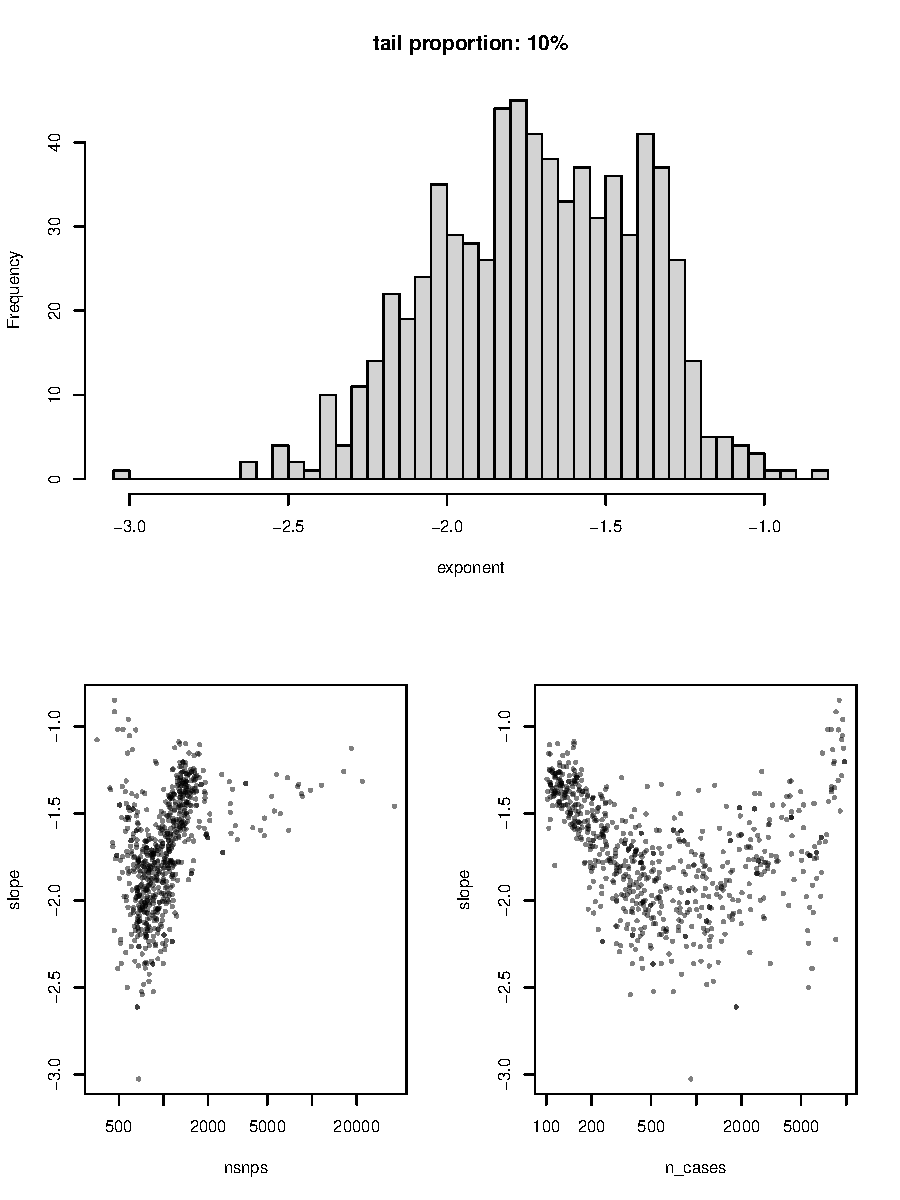
\includegraphics{snp_effects/results_10}
    \end{center}
    \caption{
        Estimated values of the tail exponent, $\alpha$,
        for 775 illness-related binary phenotypes:
        \textbf{(A)} distribution of values; and plotted against
        \textbf{(B)} number of SNPs, and
        \textbf{(C)} number of cases.
        \textbf{(D)} shows the number of SNPs and number of cases by phenotype.
        \label{fig:exponent_hist}
    }
\end{figure}

A possible concern is that tail exponents are difficult to estimate accurately, \revpoint{1}{4}
but simulation-based estimates of accuracy (Supplemental Figure~\ref{fig:power})
suggest that our estimates are unbiased but only accurate to within roughly $\pm 0.4$,
so the distribution of Figure~\ref{fig:exponent_hist} should not be taken as
a direct estimate of the underlying distribution of $\alpha$ values,
but is robust evidence for exponents strictly between 1 and 2 (and probably around 1.5).

%%%%%%%%%%%%%%%%%%%%%%
\section{Independence and the Gaussian assumption}

We know from \citet{barton2017infinitesimal} \revpoint{1}{5} \revpoint{2}{4}
that if the $\eta^{[i]}_\ell$ are
independent with mean zero and $\sum_{\ell=1}^M \var[\eta_\ell]/M \to \sigma^2$ as $M \to \infty$,
then with $\alpha \ge 2$,
the traits $(Z_M, Z_M^{[1]}, Z_M^{[2]})$ converge in distribution to a multivariate Gaussian distribution
$(Z, Z^{[1]}, Z^{[2]})$ for which $Z - (Z^{[1]} + Z^{[2]})/2$ is independent of $Z^{[1]}$ and $Z^{[2]}$.
(The main result in \citet{barton2017infinitesimal} is that the trait values in generation $t$
are Gaussian conditioned on the traits in generation $t-1$,
but as discussed in that paper,
this implies that the traits of any set of individuals is multivariate Gaussian,
with covariance matrix determined by the pedigree.
Note, however, that this does \emph{not} imply that the distribution of trait values
across the population is Gaussian, as a collection of correlated Gaussians is not itself Gaussian.)

Perhaps surprisingly, there is a converse --
in at least some situations,
independence of the Mendelian sampling term \emph{implies} a Gaussian distribution.
To see this (and to see exactly what we mean by this),
divide the parental loci into groups according to the results of inheritance,
defining
\begin{align*}
    U_M^{[1]} &= \sum_{\ell=1}^M X_\ell \eta_\ell^{[1]}  ,
    \qquad \qquad
    V_M^{[1]} = \sum_{\ell=1}^M (1-X_\ell) \eta_\ell^{[1]} ,  \\
    U_M^{[2]} &= \sum_{\ell=1}^M (1-X_\ell) \eta_\ell^{[2]} ,
    \qquad \qquad
    V_M^{[2]} = \sum_{\ell=1}^M X_\ell \eta_\ell^{[2]}  ,
\end{align*}
so that 
$Z_M^{[1]} = U_M^{[1]} + V_M^{[1]}$ and
$Z_M^{[2]} = U_M^{[2]} + V_M^{[2]}$, while
$Z_M = U_M^{[1]} + U_M^{[2]}$ is the transmitted portion of the parental genomes,
and we can define $V_M = V_M^{[1]} + V_M^{[2]}$ to be the untransmitted portion.
Furthermore,
\begin{align*}
    \bar Z_M = \frac{Z_M + V_M}{2}
    \qquad \text{ and } \qquad
    R_M = \frac{Z_M - V_M}{ 2 } .
\end{align*}

Now, note that if inheritance (the $X_\ell$) is independent of the per-locus effects ($\eta_\ell^{[i]}$),
the latter are all independent of each other,
and all effects at a given locus are drawn from the same distribution,
then the inherited allele, 
$\eta_\ell^{[1]} X_\ell + \eta_\ell^{[2]} (1-X_\ell)$
is independent of (and has the same distribution as)
the non-inherited allele,
$\eta_\ell^{[1]} (1-X_\ell) + \eta_\ell^{[2]} X_\ell$
-- they are simply two independent draws from the distribution of effects at locus $\ell$.
Therefore, the inherited alleles that sum to $Z_M$
are independent of the non-inherited alleles that sum to $V_M$.

The Kac-Bernstein theorem states that if two independent random variables
have the property that their sum and difference are independent of each other,
then the random variables have a joint Gaussian distribution
(\citet{kac1939characterization,bernstein1941property},
and see \citet{kagan1973characterization} for many much more general results).
Since $R_M$ is (half) the difference and $\bar Z_M$ is (half) the sum
of $Z_M$ and $V_M$, and $Z_M$ and $V_M$ are independent,
if we assume that also $R_M$ and $\bar Z_M$ are independent,
then both are therefore jointly Gaussian.

We have shown the following:

\begin{prop}\label{prop:parental_contribs}
    Suppose that $\{\eta_\ell^{[i]}\}$ are independent for all $\ell$ and $i$,
    that the distribution of $\eta_\ell^{[i]}$ only depends on $\ell$,
    and that $\{X_\ell\}$ are independent of $\{\eta_\ell^{[i]}\}$.
    If the Mendelian sampling term $R_M$ is independent of the midparent value $\bar Z_M$,
    then $R_M$ and $\bar Z_M$ are jointly Gaussian.
\end{prop}

We should now discuss what this counter-intuitive result says and does not say.
The proposition says, roughly, that if the parental alleles are unlinked and independently chosen,
and meotic segregation is fair,
then independence of Mendelian sampling term from midparent value
\emph{implies} a joint Gaussian distribution for the two.
We have not assumed anything about the distribution of the trait in the population:
rather, we have showed that any model of this sort
that assumes independence of Mendelian sampling term and midparent value
must also, by logical necessity, have a Gaussian distribution for the two.
In other words,
since models can be easily set up for which the distribution of Mendelian sampling terms
is not Gaussian,
the implication of the proposition
is that for such models, independence of the Mendelian sampling term
is not likely a good assumption. \revpoint{1}{7}
Note that the proof does not depend on independence of the $X_\ell$:
indeed, alleles may be inherited together,
although in practice this would quickly create dependencies between the effects
of alleles at such linked loci. \revpoint{2}{5}
Also note that it is \emph{not} usually true that the components --
for instance, $U_M^{[1]}$ and $U_M^{[2]}$ --
are independent of each other.
Finally, note that although they may not be independent,
the Mendelian sampling term $R_M$ and the midparent value $\bar Z_M$
\emph{are} always uncorrelated, since $Z_M$ and $V_M$ are exchangeable.

Note that under the conditions of the proposition, \llabel{pop_not_gaussian}
the parental traits, $Z^{[1]}_M$ and $Z^{[2]}_M$,
are also (jointly) Gaussian.
(This was not an assumption, however.)
If parents are chosen uniformly, then
the distribution of, say, $Z^{[1]}$ is just the population's trait distribution.
This seems wrong, since it is well-known that forces such as selection or migration
can make the population distribution non-Gaussian.
However, there is no contradiction:
we have stated the proposition only in terms of the \emph{first} generation
of offspring of unrelated parents \citep[as in][]{barton2017infinitesimal}.
Proposition~\ref{prop:parental_contribs} does not imply that
the distribution of traits in the offspring generation is Gaussian:
unless all offspring are unrelated,
it will be a collection of correlated Gaussians,
which is not itself Gaussian.
(As an extreme example, suppose that half the offspring are produced by the two parents
with largest trait values, and the other half by the parents with the smallest trait values;
then although each offspring's distribution about the midparent is Gaussian,
the offspring's population distribution is a mixture of two Gaussians
about these two midparents.)
What about further generations?
A similar statement to the proposition
holds for the offspring of two parents in an arbitrary pedigree,
using the Skitovich-Darmois theorem \citet{kagan1973characterization}
% except that the portion of the genome shared in common by the parents is unconstrained.
-- however, there is nothing to be gained by the additional generality.

As we discuss more later,
the presence of a large effect allele at a polymorphic locus \llabel{loci_polymorphic}
makes $R$ and $\bar Z$ dependent:
consider the extreme case where $\eta^{[i]}_\ell$ are i.i.d.{} with variance 1 for $\ell \ge 2$,
while $\eta^{[i]}_1 = \pm 10$ with probability 1/2 each,
and $Z^{[i]} = \eta_1^{[i]} + \sum_{\ell=2}^M \eta_\ell^{[i]} / \sqrt{M}$.
Then in the limit $R$ depends strongly on parental trait values:
if $Z^{[1]} \approx Z^{[2]}$ and so $\bar Z \approx \pm 10$ then most likely
$\eta_1^{[1]} = \eta_1^{[2]}$ and so $R$ is Normal with variance 1/2;
but if $\eta_1^{[1]} \neq \eta_1^{[2]}$ (and so $\bar Z \approx 0$)
then $R$ is close to $+5$ or $-5$ with equal probability.

Finally, a possible point of confusion is that \revpoint{1}{6}
the infinitesimal model is often phrased as a statement about offspring trait distributions
\emph{given} parental trait values,
while our statement above regards parental trait values as random.
However, the notions are equivalent:
the statement that
``for each pair of parents the deviation of the offspring's trait from midparent
has a distribution that does not depend on the parents' values''
is essentially the definition of statistical independence
of offspring's Mendelian sampling term and parental trait values.

%%%%%%%%%%%%%%%%%%%%%%
\section{Abnormal quantitative genetics?}

As observed in \cite{turelli2017commentary}, \revpoint{1}{8}
there are at least three interpretations of what is called ``the infinitesimal model''.  The maximalist of these, what \cite{turelli2017commentary} calls the Gaussian-population approximation, assumes a large number of small-effect loci,  parental trait-independent Gaussian Mendelian sampling terms  (as rigorously justified in \cite{barton2017infinitesimal,barton2022infinitesimal}), and, moreover, that  population trait values are in deterministic mutation-selection balance, with a Gaussian empirical distribution
(\ie the \emph{fraction} of the population with trait value in $[z,z+dz)$
is approximately $\frac{1}{2\pi\sigma^{2}} e^{-(z-m)^{2}/(2\sigma^{2})} dz$
for suitable choices of the empirical mean and variance $m$ and $\sigma^{2}$).
Leaving aside
% -- as the Gaussian-population approximation frequently does --
the question of whether or not some combination of effect sizes, dominance, and epistasis can justify non-Gaussian, trait-independent,  Mendelian sampling terms, we might reasonably ask when (or if)
deterministic mutation-selection balance is possible in a non-Gaussian model
that retains independence of the Mendelian sampling terms.
(Indeed, above we have put substantial restrictions on what models of inheritance
might lead to such models.)
We might also ask whether such a model
might still reasonably approximate an additive model with non-Gaussian effects,
and for the purpose of investigating this with simulations,
some calculations will be helpful.

Concretely, consider a  Moran process where an individual whose trait value is $Z$ dies at rate $\mu(Z)$
and is replaced by the offspring of two randomly chosen individuals,
i.e., a new individual with trait
\begin{align*}
  \frac{Z^{1} +Z^{2}}{2} + R ,
\end{align*}
where $Z^{1}$ and $Z^{2}$ are independent draws from the empirical population distribution
and $R$ is an independent draw from the Mendelian sampling distribution
(independent of $Z^{1}$ and $Z^{2}$, with distribution to be specified). 
Mutation-selection balance demands that that
the distribution of individuals removed by death
and the distribution of individuals added by birth are equal,
\ie that $(Z^{1} +Z^{2})/2 + R$ is equal in distribution
to a $\mu$-weighted choice of $Z$.
% In other words, for all bounded and continuous functions $f$,
% \begin{equation} \label{eqn:MSB_condition}
%     \E\left[ f\left(\frac{Z^{1} +Z^{2}}{2} + R \right) \right] = \frac{\E\left[ f(Z) \mu(Z) \right]}{\E[\mu(Z)]},
% \end{equation}
% where the expectation is with respect to the joint law of the population empirical distribution (the law of $Z$, $Z^{1}$ and $Z^{2}$), and $R$.
% 
% Since the set of functions $\mathcal{S} = \{e^{i \theta x} : \theta \in \R\}$ is separating (see \eg \S 3.4 in \cite{Ethier+Kurtz1986}), it suffices to show that \eqref{eqn:MSB_condition} holds for $f \in \mathcal{S}$, \ie
Taking the characteristic function of both these distributions,
deterministic mutation-selection balance is therefore equivalent to
\begin{align} \label{eqn:MSB_CF}
    \frac{\E\left[ e^{i \theta Z}\mu(Z) \right]}{\E[\mu(Z)]}
    =
    \E\left[ e^{i\theta\left(\frac{Z^{1} +Z^{2}}{2} + R \right)}\right] .
\end{align}
Now, we assumed that $Z^{1}$, $Z^{2}$, and $R$ are independent, so we can write \eqref{eqn:MSB_CF} as 
\begin{align*}
    \frac{\E\left[ e^{i\theta Z} \mu(Z) \right]}{\E[\mu(Z)]} &= \E\left[ e^{i\theta\left(\frac{Z^{1} +Z^{2}}{2} + R \right)}\right]\\
	% &= \E\left[ e^{i\frac{\theta}{2} Z^{1}}e^{i\frac{\theta}{2} Z^{2}}e^{\i\theta R}\right]\\
	&= \E\left[e^{i\frac{\theta}{2} Z^{1}}\right]\E\left[e^{i\frac{\theta}{2} Z^{2}}\right]\E\left[e^{i\theta R}\right]\\
	&= \phi\left(\frac{\theta}{2}\right)^{2} \Phi(\theta),
\end{align*}
where
$ \phi(\theta) = \mathbb{E}\left[e^{i\theta Z^{1}}\right] = \mathbb{E}\left[e^{i\theta Z^{2}}\right] $
and
$ \Phi(\theta) = \mathbb{E}\left[e^{i\theta R}\right] $
are the characteristic functions of $Z^{j}$ and $R$, respectively.  In what follows, we will explore some non-Gaussian solutions $\phi(\theta)$ to \eqref{eqn:MSB_CF}.

\subsection{The Neutral Case}

First, consider the case without selection, so $\mu$ is a constant
which we may take equal to 1.  Then, our condition on the characteristic function simplifies to
\begin{equation}\label{eq:CF_neutral}
	{\textstyle \phi\left(\frac{\theta}{2}\right)^{2}} \Phi(\theta) %e^{-\frac{\eta^{2}\theta^{2}}{2}} 
	= \phi(\theta) ,
\end{equation}
\ie $\phi(\theta)$ is a fixed point of $F$, where
 \[
	F(\phi)(\theta) = {\textstyle \phi\left(\frac{\theta}{2}\right)^{2}} \Phi(\theta),
\]
whereas any fixed point must be the limit of an arbitrary characteristic function, $\varphi(\theta)$, under repeated applications of $F$,
\ie \revpoint{2}{7}
\begin{align*}
	\phi(\theta) 
    &= \lim_{n \to \infty} F^{(n)}(\varphi)(\theta) \\
    &= \lim_{n \to \infty} \varphi\left(\frac{\theta}{2^{n}}\right)^{2^{n}}\prod_{k=1}^{n-1}\Phi\left(\frac{\theta}{2^{k}}\right)^{2^{k}} .
\end{align*}
% Iterating $F$ $n$ times, we get
% \[
% 	F^{(n)}(\varphi)(\theta) =  {\textstyle \varphi\left(\frac{\theta}{2^{n}}\right)^{2^{n}}}\prod_{k=1}^{n-1} {\textstyle \Phi\left(\frac{\theta}{2^{k}}\right)^{2^{k}}},
% \]
% so that
% \[
% 	\phi(\theta) = \lim_{n \to \infty} \varphi\left(\frac{\theta}{2^{n}}\right)^{2^{n}}\prod_{k=1}^{n-1}\Phi\left(\frac{\theta}{2^{k}}\right)^{2^{k}}
% \]
is a fixed point whenever this limit exists.  

Since $\varphi$ and $\Phi$ are characteristic functions, they are continuous and $\phi(0) = \Phi(0) = 1$, and thus both are non-zero in a neighbourhood of 0. In particular, $\psi(\theta) = \Log{\varphi}(\theta)$ and $\Psi(\theta) = \Log{\Phi(\theta)}$ exist in some neighbourhood of 0 as well\footnote{We use $\Log$ to denote the principal value of the complex logarithm, for which the imaginary part always lies in the interval $(-\pi,\pi]$.}.  From the above, we have
\[
	\Log{F^{(n)}(\varphi)(\theta)} = {\textstyle 2^{n} \psi\left(\frac{\theta}{2^{n}}\right)} 
		+ \sum_{k=1}^{n-1}  {\textstyle 2^{k} \Psi\left(\frac{\theta}{2^{k}}\right)}.
\]
We briefly explore what possible limiting values are valid characteristic functions.  We refer to the first term on the left hand side as the \emph{reproduction term} and the remaining sum as the \emph{noise term}, and only consider to the case when both have well-posed limits independent of the other. \llabel{limit_remark}

\paragraph{Noise Terms}
First, consider the noise terms.  A necessary condition for $\sum_{k=1}^{\infty} 2^{k} \Psi\left(\frac{\theta}{2^{k}}\right)$ to converge is that $2^{k} \Psi\left(\frac{\theta}{2^{k}}\right) \to 0$; since $\Psi(0) = 0$, this implies that if it exists, $\Psi'(0+) = 0$.  In particular, as we would expect, if $R$ has a mean, it must be 0.  If, on the other hand, $\Psi(\theta)$ is twice differentiable, so $R$ has mean 0 and finite variance, say $\Psi''(0) = \eta^{2}$, then Taylor's theorem tells us that for $\theta$ sufficiently small, 
\[
	\Psi(\theta) = \frac{\eta^{2}}{2} \theta^{2} + r(\theta)\theta^{2},
\]
where $r(\theta) \to 0$ as $\theta \to 0$.  Thus,
\begin{equation*}
	\frac{\textstyle 2^{k+1} \Psi\left(\frac{\theta}{2^{k+1}}\right)}{\textstyle 2^{k} \Psi\left(\frac{\theta}{2^{k}}\right)}
	= \frac{1}{2} \frac{\eta^{2} \theta^{2} + {\textstyle  r\left(\frac{\theta}{2^{k+1}}\right)}\theta^{2}}{\eta^{2} \theta^{2} + {\textstyle  r\left(\frac{\theta}{2^{k}}\right)}\theta^{2}}
	\to \frac{1}{2},
\end{equation*}
as $k \to \infty$ and the sum converges by the ratio test.  In this case,
\begin{align*}
	 \sum_{k=1}^{n-1}  {\textstyle 2^{k} \Psi\left(\frac{\theta}{2^{k}}\right)}
	 &=  \sum_{k=1}^{n-1} 2^{k} {\textstyle \left(- \frac{\eta^{2}}{2}  \frac{\theta^{2}}{2^{2k}}
		+ r\left(\frac{\theta}{2^{k}}\right)\frac{\theta^{2}}{2^{2k}}\right)}\\
	&=- \eta^{2} \theta^{2} (1 - 2^{-n+1})  + \sum_{k=1}^{n-1} {\textstyle r\left(\frac{\theta}{2^{k}}\right)\frac{\theta^{2}}{2^{k}}}
\end{align*}
If we assume that $r(\theta) \equiv 0$, so that the noise is $N(0,\eta^{2})$, then the limiting distribution is $N(0,2\eta^{2})$. When  $r(\theta)$ is non-zero, we don't expect the higher order terms to vanish.

It is unclear what more can be said in general. If however, we specialize to the case when $R$ is a stable law, we can explicitly compute the limiting noise term.  We recall that if $\Psi(\theta)$ corresponds to a stable law (see \eg \cite{breiman1992probability}), then
\[
	\Psi(\theta) = im\theta - c|\theta|^{\alpha} (1-i\beta \sgn(\theta)\omega_{\alpha}(\theta))
\]
for $\alpha \in (0,2]$, $\beta \in [-1,1]$, $c \geq 0$, and $m \in \mathbb{R}$ and
\[
	\omega_{\alpha}(\theta) = \begin{cases}
		\tan{\frac{\pi\alpha}{2}} & \text{if $\alpha \neq 1$, and}\\
		-\frac{2}{\pi}\log{|\theta|} & \text{if $\alpha = 1$.}
	\end{cases}
\]
By our general remarks above, we can assume $m = 0$ and exclude the case $\alpha = 1$, $\beta = 0$, for which  $\Psi'(0+) = c$. We then have
\begin{align*}
	 \sum_{k=1}^{n-1}  {\textstyle 2^{k} \Psi\left(\frac{\theta}{2^{k}}\right)}
	 &=  \sum_{k=1}^{n-1} -2^{(1-\alpha)k} c|\theta|^{\alpha} {\textstyle\left(1-i \beta\sgn\left(\frac{\theta}{2^{k}}\right)
	 	 \omega_{\alpha}\left(\frac{\theta}{2^{k}}\right)\right)}\\
	&= \begin{cases}
		 -c|\theta|^{\alpha}\frac{1-2^{(1-\alpha)n}}{1-2^{1-\alpha}}\left(1-i\beta \sgn(\theta) \tan{\frac{\pi\alpha}{2}}\right) & \text{if $\alpha \neq 1$, and}\\	
         -(n-1) c|\theta| \left(1+\frac{2i\beta}{\pi}\sgn(\theta)\left(\log{|\theta|} - \frac{n}{2} \log{2}\right)\right) & \text{if $\alpha = 1$,}
	\end{cases}
\end{align*}
which converges as $n \to \infty$ if and only if $\alpha > 1$, in which case the limit is 
\begin{equation}\label{eq:stablenoises}
	 -\frac{c}{1-2^{1-\alpha}}|\theta|^{\alpha}\left(1-i\beta \sgn(\theta) \tan{\frac{\pi\alpha}{2}}\right), 
\end{equation}
which corresponds to a $\left(\alpha,\beta, \frac{c}{1-2^{1-\alpha}},0\right)$-stable law.

\paragraph{Reproductive Terms:}
We now turn our attention to the limit
\[
		\alpha(\theta) = \lim_{n \to \infty} 2^{n}\psi\left(\frac{\theta}{2^{n}}\right)
\]
If it exists, then for all integers $k$, 
\[
	\alpha(2^{k} \theta) = \lim_{n \to \infty} 2^{n}\psi\left(\frac{2^{k} \theta}{2^{n}}\right) =  \lim_{n \to \infty} 2^{k} 2^{n-k} \psi\left(\frac{\theta}{2^{n-k}}\right) = 2^{k} \alpha(\theta).
\]
and, since $\alpha(0) = 0$,
\[
	\frac{\alpha(\theta)}{\theta} = \frac{\alpha(2^{k} \theta)}{2^{k}\theta} 
	\to \begin{cases} 
		\alpha'(0+) & \text{if $\theta > 0$, and}\\
		\alpha'(0-) & \text{if $\theta < 0$,}
	\end{cases}
\]
as $k \to - \infty$ if the limits exist (\ie there are unique left-and right-hand limits at zero; this is the case if \eg we require $\alpha(\theta)$, and thus $\phi(\theta)$, to be convex functions).  We henceforth assume this.

Since $\varphi(\theta)$ is a characteristic function, it has the Hermitian property: $\phi(-\theta) = \overline{\phi(\theta)}$, and thus $\psi(-\theta) = \overline{\psi(\theta)}$ and $\alpha(-\theta) = \overline{\alpha(\theta)}$.  In particular, if one (and by extension both) limits exist, we must have $\alpha'(0-) = \overline{\alpha'(0+)}$.  In this case, setting $-\gamma + i m = \alpha'(0+)$, we have
\[
	\alpha(\theta) = \begin{cases} 
		i m\theta - \gamma \theta & \text{if $\theta \geq 0$, and}\\
		i m\theta + \gamma \theta & \text{if $\theta < 0$}.
	\end{cases}
\]
If $\gamma > 0$, then we recognize $e^{\alpha(\theta)} = e^{im \theta -\gamma|\theta|}$ as the characteristic function of a Cauchy distribution with median 0 and median absolute deviation $\gamma$, whereas if $\gamma = 0$, then $e^{\alpha(\theta)} = e^{im \theta}$ is the Fourier transform of a Dirac mass at $m$, \ie the characteristic function for a monomorphic population with all individuals having trait value equal to $m$.
(And, $\gamma < 0$ does not give a valid characteristic function.)
% % I think we've shown this characteristic function has to be exp(im\theta - \gamma|\theta|);
% % if $\gamma < 0$ then it is not a characteristic function; am I missing something?
% In general, it does not seem possible to exclude $\gamma < 0$. However, recalling that if $\phi(\theta)$ is the characteristic function of a random variable $Z$, Jensen's inequality tells us that for all $\theta$,
% \begin{equation}\label{eq:CF-J}
% 	|\phi(\theta)| = \left|\E\left[e^{i\theta Z}\right]\right| \leq \E\left[\left|e^{i\theta Z}\right|\right] = 1,
% \end{equation}
% we can conclude $\gamma \geq 0$ when the limiting noise term is a mixture of Gaussians and stable laws of the form \eqref{eq:stablenoises}: we then have 
% \[
% 	|\phi(\theta)| = e^{\re(\alpha(\theta) + o(|\theta|))} = e^{\gamma |\theta| + o(|\theta|))},
% \] 
% and thus is less than or equal to one in a small neighbourhood of $0$ if and only if $\gamma < 0$.

\paragraph{Blending inheritance redux.} 
Note that the characteristic functions constructed above are solutions to \eqref{eq:CF_neutral} when transmission is noiseless, and the offspring have exactly the parental mean trait -- \ie blending inheritance.  The solution $\phi(\theta) = e^{i\theta m}$ is exactly the reversion to the mean that Darwin's detractors used to argue against the theory of evolution \citep{jenkin1867,Provine1971}.  The solution $\phi(\theta) = e^{im \theta -\gamma|\theta|}$ offers an amusing counter-factual: if a Lamarkian population could somehow achieve a Cauchy-distributed trait distribution, it would maintain that diversity indefinitely.  

% \paragraph{Other solutions?}
% We would naturally like to know if these two exhaust the possible solutions.  Above, we exhausted all solutions for which $\alpha'(0+)$ exists.  However, if $\frac{\alpha(\theta)}{\theta}$ is non-constant for $\theta > 0$, then $\alpha'(0+)$ does not exist. This does not, however, in and of itself exclude $e^{\alpha(\theta)}$ from being a characteristic function: Bochner's theorem tells us that a function $\phi(\theta)$ is the characteristic function of a random variable if and only if
% \begin{enumerate}[(i)]
% \item $\phi(\theta)$ is continuous,
% \item $\phi(0) = 1$,
% \item $\phi(-\theta) = \overline{\phi(\theta)}$, and
% \item $\phi(\theta)$ is \textit{positive definite}: for all $n$ and all $\theta_{1},\ldots,\theta_{n} \in \mathbb{R}$, the matrix with entries $a_{ij} = \phi(\theta_{i}-\theta_{j})$
% \end{enumerate}
% One can easily choose $\alpha(\theta)$ so that $e^{\alpha(\theta)}$ satisfies the first three criteria, \eg $\alpha(\theta) = -|\theta|\left(\sin\left(\pi\frac{\log{|\theta|}}{\log{2}}\right)+\frac{3}{2}\right)$, but excluding such functions via Bochner's positive definite criterion is non-trivial.



More generally, one will get convergence if the noise is a mixture of components with finite variance and stable laws as above, whereas the population distribution will be a mixture of a (possibly degenerate) Cauchy distribution and such noise terms. Note that in the presence of noise, a pure Cauchy-distributed solution is \emph{not} possible in the neutral case.

\subsection{Stabilizing Selection}
    \label{sec:stabilizing_selection}
    
Unfortunately, once selection is included, \eqref{eqn:MSB_CF} is less amenable to the sort of simple arguments above.  We will content ourselves with presenting two examples of stabilizing selection, one already familiar to quantitative genetics, the other a Cauchy solution obtained by trial-and-error, which illustrates how selection can stabilize an otherwise unviable solution.

\paragraph{Gaussian Solution:}
First, consider the case when $\mu(x) = e^{a x^{2}}$.   In this case there is a Gaussian solution: suppose $Z$ is Gaussian with mean $m$ and variance $\sigma^{2}$, so
$ \phi(\theta) = \exp(i m \theta - \frac{1}{2} \sigma^{2} \theta^{2}).  $
Moreover, provided $a < \frac{1}{2\sigma^{2}}$, we can explicitly compute $\frac{\mathbb{E}\left[e^{i \theta Z}\mu(Z)\right]}{\mathbb{E}[\mu(Z)]}$: %  using the Gaussian probability density function to conclude that
if $R$ is Gaussian with mean zero and variance $\eta^2$, then equation~\eqref{eqn:MSB_CF} becomes
\[
	e^{i m \theta - \frac{1}{2} \left(\frac{\sigma^{2}}{2} + \eta^{2}\right)\theta^{2}}
	= e^{i \frac{m}{1-2 a \sigma^{2}}\theta 
		- \frac{1}{2} \frac{\sigma^{2}}{1-2 a \sigma^{2}}\theta^{2}},
\]
which, equating real and complex components, has a solution provided $m = 0$ and
\[
	\sigma^{2} = \frac{\sqrt{16 a^{2} \eta^{4} + 24 a \eta^{2}+1} - 4a \eta^{2} -1}{4a} 
	=  2\eta^{2}(1-4a\eta^{2}) + O(a^{2}).
\]

Note that we do not require very weak selection to guarantee a Gaussian steady state, only that $a < \frac{1}{4\eta^{2}}$.  However, this does not imply that the transient distribution is also Gaussian, as is sometimes assumed \citep[e.g.,][]{lande1976natural}. %  The latter does indeed require very weak selection.


\subsubsection{Cauchy Solution}
    \label{sec:stabilizing_cauchy}

Almost uniquely among the stable laws, the Cauchy distribution has a probability density function expressible in elementary functions: 
% (the other exceptions being the L\'evy and Gaussian distributions): 
for a Cauchy random variable with median (location) $x_{0}$ and mean absolute deviation (scale) $\gamma$, the density is 
\begin{equation}\label{eq:Cpdf}
	f(x;x_{0},\gamma) = \frac{1}{\pi\gamma\left[1+\left(\frac{x-x_{0}}{\gamma}\right)^{2}\right]}.  
\end{equation}	
Armed with this density function, we can explicitly compute the right hand size of \eqref{eqn:MSB_CF}, assuming that 
\begin{enumerate}[(i)]
\item the population is in mutation-selection balance corresponding to a Cauchy density with median 0 and scale $\gamma > 0$,
\item selection acts as $\mu(x) = \frac{\delta^{2}}{\gamma^{2}} \frac{\gamma^{2} + x^{2}}{\delta^{2} + x^{2}}$ for some $\delta > \gamma > 0$, and
\item the Mendelian sampling term $R$ is given by a $\text{Cauchy}(0,\delta-\gamma)$ random variable (\ie corresponding to a stable $(1,0,\delta-\gamma,0)$ law).
\end{enumerate}

Under these assumptions, \eqref{eqn:MSB_CF} is
\begin{align*}
	\frac{\mathbb{E}\left[e^{i \theta Z}\mu(Z)\right]}{\mathbb{E}[\mu(Z)]} 
	&= e^{-\delta |\theta|}\\
	&= e^{-2\gamma \left|\frac{\theta}{2}\right|-(\delta-\gamma)|\theta|},
\end{align*} 
which we recognize as being equal to $\phi\left(\frac{\theta}{2}\right)^{2} \Phi(\theta)$, where $\phi(\theta) = e^{i\gamma|\theta|}$ and $\Phi(\theta) = e^{i(\delta - \gamma)|\theta|}$ are the characteristic functions of the population density and the Mendelian sampling term, respectively,
giving a.non-Gaussian solution to \eqref{eqn:MSB_CF} with both noise and selection.

As remarked above, we found this solution by inspection and trial-and-error; it is interesting to ask if any similar examples can be constructed for other stable laws.  The lack of an elementary probability density function unfortunately rules out the na\"ive approach used here. 

%(here, see a saturating cost to being away from the optimal phenotype $x = 0$: the mortality is maximized at  $\frac{\beta^{2}}{\alpha^{2}}$.

\section{The difficulty with an abnormal quantitative genetics}

Above we have seen that
(a) in principle,
a mutation-selection balance is possible with a Cauchy empirical distribution and Cauchy Mendelian noise,
but (b)
such a model cannot derive from a simple model of additive loci.
To that end, it's instructive to see where the argument of \cite{barton2017infinitesimal} breaks down
if instead of assuming bounded allele effects of order $\Oh(1/\sqrt{M})$,
we assume that the allele at locus $\ell$ in individual $j$ contributes
$\eta^{[j]}_{\ell}/M$, where the $\eta^{[j]}_{\ell}$ are independent $\Cauchy(0,\gamma_{\ell})$ random variables. 
In this case, the typical effect size at locus $\ell$ is of order $\frac{\gamma_{\ell}}{M}$,
which is asymptotically smaller than the allele effects assumed in \cite{barton2017infinitesimal},
but large effect alleles are more likely. 

The crucial step in the derivation of the infinitesimal model in \cite{barton2017infinitesimal} is to show that, following the arguments in \cite{Fisher1918}, knowing an individual's trait value gives vanishingly little information about the contribution of any given locus as $M \to \infty$, which in turn allows one to show that the within-family Mendelian segregation variance is independent of the parental traits. Here, we will consider how conditioning an individual's trait value affects the law of a single allelic contribution in the Cauchy setting described above. A similar argument can be made for any $\alpha$-stable distribution, but the lack of explicit probability density functions for generic $\alpha \in (0,2)$ adds complexity to the argument without adding any insight. 

% The key observation is this:
% while is meaningless to speak of variances when the Mendelian sampling term is $\alpha$-stable, if an individual's trait value is informative of the allelic effect at any given locus,
% then its trait value is informative of the \emph{distribution} of an offsprings' trait value,
% and hence there can be no independence between parental traits and the Mendelian sampling term
% that is central to the tractability of the infinitesimal model.  

Consider the simplest possible case of an ancestral population, of $N$ individuals, where the $j$\textsuperscript{th} individual has trait value 
\[
	Z^{[j]}_{M} = \frac{1}{M} \sum_{\ell = 1}^{M}  \eta^{[j]}_{\ell},
\]
where the $\eta^{[j]}_{\ell}$ are independent across individuals and across loci.  By the additive property of Cauchy random variables, $Z^{[j]}_M \iid \Cauchy(0,\bar{\gamma})$, where 
\[
	\bar{\gamma} = \frac{1}{M} \sum_{\ell = 1}^{M} \gamma_{\ell}
\]
is the mean of the scale parameters.  

To see what knowing the parental trait value $Z^{[j]}_{M}$ \revpoint{1}{16}
tells us about the contribution of any given locus, $\eta^{[j]}_{\ell}$, we follow the arguments in  \citet{Fisher1918} and \citet{barton2017infinitesimal} using Bayes' Theorem. Proceeding informally, with the probabilities indicating probability density functions, we have 
\begin{align*}
    \P\{\eta^{[j]}_{\ell} = y \vert Z^{[j]} = z\} &= \frac{\P\{\eta^{[j]}_{\ell} = y; Z^{[j]} = z\}}{\P\{Z^{[j]} = z\}}\\
        &= \frac{\P\{Z^{[j]} = z\vert\eta^{[j]}_{\ell} = y\}}{\P\{Z^{[j]} = z\}}\P\{\eta^{[j]}_{\ell} = y\}\\
        &=  \frac{\P\{Z^{[j]} -\frac{1}{M} \eta^{[j]}_{\ell} = z - \frac{1}{M} y\}}{\P\{Z^{[j]} = z\}}\P\{\eta^{[j]}_{\ell} = y\}\\
\end{align*}
Now, $Z^{[j]} -\frac{1}{M} \eta^{[j]}_{\ell} = \frac{1}{M} \sum_{k = 1 : k \neq i}^{M} \eta^{[j]}_{k}$ is Cauchy-distributed with scale $\bar{\gamma} - \frac{\gamma_{\ell}}{M}$.  Using the probability density function for a Cauchy distributed random variable \eqref{eq:Cpdf}, a straightforward computation gives
\begin{align*}
    \P\{\eta^{[j]}_{\ell} = y \vert Z^{[j]} = z\}
    &=
    \frac{f\left(z - \frac{y}{M} ;0,\bar{\gamma}-\frac{\gamma_{\ell}}{M}\right)}{f(z;0,\bar{\gamma})} \P\{\eta^{[j]}_{\ell} = y\}\\
    &=
    \left(1
        +
        \frac{\gamma_{\ell}(\bar{\gamma}^{2}-z^{2})+2zy}{\gamma_{\ell}(\bar{\gamma}^{2}+z^{2})}
        \frac{1}{M}
        + \Oh\left(\frac{1}{M^{2}}\right)\right)
        \P\{\eta^{[j]}_{\ell} = y\}.
\end{align*}
Noting that $|(\bar{\gamma}^2 - z^2)/(\bar{\gamma}^2 + z^2)| \le 1$
and $|z/(\bar{\gamma}^2 + z^2)| \le 1/(2 \bar{\gamma})$
(since it is maximized at $z = \bar{\gamma}$),
so
\begin{align*}
        \left|
        \frac{\gamma_{\ell}(\bar{\gamma}^{2}-z^{2})+2zy}{\gamma_{\ell}(\bar{\gamma}^{2}+z^{2})}
        \right|
        \le \frac{|y|}{\gamma_\ell \bar{\gamma}} ,
\end{align*}
% Now, as $z \to 0$,
% $\frac{\gamma_{\ell}(\bar{\gamma}^{2}-z^{2})+2zy}{\gamma_{\ell}(\bar{\gamma}^{2}+z^{2})} \to \frac{\gamma_{\ell}}{\bar{\gamma}}$
% and as $z \to \pm \infty$,
% $\frac{\gamma_{\ell}(\bar{\gamma}^{2}-z^{2})+2zy}{\gamma_{\ell}(\bar{\gamma}^{2}+z^{2})} \to -\frac{\gamma_{\ell}}{\bar{\gamma}}$,
% \comment{I'm not sure where $\gamma_\ell$ went here}
% whereas $|\frac{\bar{\gamma}^{2}-z^{2}+2zy}{\bar{\gamma}^{2}+z^{2}}|$ 
% \[
% 	\frac{(\gamma_{\ell}^{2}+y^{2})\left(\sqrt{\gamma_{\ell}^{2}+y^{2}}-\gamma_{\ell}\right)}{\bar{\gamma}(\gamma_{\ell}^{2}+y^{2} - \gamma_{\ell}\sqrt{\gamma_{\ell}^{2}+y^{2}})},
% \]
% which is asymptotically equal to $\frac{|y|}{\bar{\gamma}}$ for large values of $|y|$, at
% \[
% 	z = -\frac{\bar{\gamma}}{y}(\gamma_{\ell} \pm \sqrt{\gamma_{\ell}^{2}+y^{2}}),  
% \]
% which is itself asymptotically equal to $\mp \sgn(y) \bar{\gamma}$ for large values of $|y|$.
we have that
\[
    \left|
    \P\{\eta^{[j]}_{\ell} = y \vert Z^{[j]} = z\} - \P\{\eta^{[j]}_{\ell} = y\}
    \right|
    \le \left(\left(1 + \frac{|y|}{\gamma_\ell \bar{\gamma}}\right) \frac{1}{M} + \Oh\left(\frac{1}{M^2}\right)\right)  \P\{\eta^{[j]}_{\ell} = y\}.
\]
% Unlike the case of bounded allelic effects, the bound is independent of the trait value $Z^{[j]}$. 
In the case of bounded allelic effects, the error introduced by approximating the effect-size distribution conditional on the trait value by the unconditioned distribution is proportional to $|Z^{[j]}|$, so that extreme trait values are most informative of the size of allelic effects,
whereas here,
the bound is independent of the trait value,
and the error is maximized when the trait value is approximately equal to
the mean absolute deviation of its distribution, \ie the median value of $|Z^{[j]}|$.

The argument above shows for a typical locus, the effect of conditioning on the trait gives negligible information about the contribution from that site.   Recalling that
\[
    \P\left\{|\eta^{[j]}_{\ell}| > y\right\} =  1-\frac{2}{\pi} \arctan\left(\frac{y}{\gamma_{\ell}}\right) \sim \frac{2\gamma_{\ell}}{\pi y},
\]
we see that for any $\epsilon > 0$, and large values of $M$,
\[
    \P\left\{\frac{\eta^{[j]}_{\ell}}{\gamma_\ell \bar{\gamma} M} > \epsilon\right\} \sim \frac{2\gamma_{\ell}}{\pi \gamma_\ell \bar{\gamma} M \epsilon}.
\]
so the probability the error is larger than $\epsilon$ at any given locus decays rapidly as $M \to \infty$. 

If, however, we consider not any one locus, but rather all loci, we get a different picture. 
The variables $\eta^{[j]}_{\ell}$ are independent, and thus so are the Bernoulli random variables 
\begin{equation}
	\1^{M}_{\ell} = \begin{cases}
        1 & \text{if $\frac{\eta^{[j]}_{\ell}}{\bar{\gamma} M} > \epsilon$, and}\\
		0 & \text{otherwise.}
	\end{cases}
\end{equation}
Now, since
\[
	\lim_{M \to \infty} \sum_{\ell = 1}^{M} \frac{2\gamma_{\ell}}{\pi \bar{\gamma} M \epsilon} = \frac{2}{\pi \epsilon},
\]
the number of loci at which the magnitude of the effect size exceeds $M \epsilon$, which is 
$\sum_{\ell = 1}^{M} \1^{M}_{\ell}$,
converges weakly as $M \to \infty$ to a Poisson random variable with mean $2/(\pi \epsilon)$ (see \eg Theorem 2.6.1 in \cite{Durrett2005}).  In particular, for large values of $M$ and fixed $\epsilon > 0$,
\begin{align*}
    \P\left\{\max_{i=1}^{M} \frac{\eta^{[j]}_{\ell}}{\bar{\gamma} M} > \epsilon\right\}  \sim 1-e^{-\frac{2}{\pi \bar{\gamma} \epsilon}},
\end{align*}
which approaches 1 as $\epsilon \to 0$, while the expected number of $M$ alleles such that $\frac{\eta^{[j]}_{\ell}}{\bar{\gamma} M} > \epsilon$ is asymptotically $\frac{2}{\pi\epsilon}$. 

In particular, there is at least one locus at which knowing the parental trait gives one information about the effect size (and there are on the order of $\Oh\left(\frac{1}{\epsilon}\right)$ that give ``an $\epsilon$ of information''), and these large effect loci in turn give rise to correlations between
parental traits and the deviation of the offsprings' traits from the midparent
(i.e., the Mendelian sampling terms).
However, the first calculations above
suggest that for ``most'' loci,
this is not true,
and so perhaps a reasonable picture of Mendelian sampling terms
in an additive model with Cauchy-distributed effects
might be ``some large Mendelian alleles plus Gaussian noise''.
We now turn to simulation,
to investigate.

%%%%%%%%%%%%%%%%%%%%%%
\section{Simulations}

In simulation we can easily include realistic recombination (instead of unlinked loci) and selection.
We used SLiM v4 \citep{haller2022slim4}
to simulate a discrete-time approximation to the continuous-time Moran model described above
as follows.
Individuals are diploid, hermaphroditic, and sexual;
the genome is of length $10^8$bp with a uniform recombination rate of $10^{-8}$ crossovers per bp;
mutations occur at a rate of $10^{-9}$ per bp.
Each new mutation is independently assigned an ``effect''
drawn from the ``effect size distribution'' (and will be either Gaussian or Cauchy).
The trait of each individual is determined additively
by summing the effects of all mutations they carry across both chromosomes.
Let $\mu(z)$ be the death rate of an individual with trait $z$,
and let $dt$ be a small constant (we took $dt=0.01$).
In all plots, one time unit is approximately one generation.
Then, at each time step
each individual dies with probability $1 - \exp(-dt \mu(z))$;
if there are $k$ such individuals chosen to die in a given time step,
then we choose $k$ individuals uniformly and without replacement
to produce new offspring;
for each such reproduction event the parent chooses a mate uniformly at random from the population.
This maintains the population at a fixed size, $N$.
(Note that individuals may self and individuals chosen to die may also reproduce,
but in a large population these details should be unimportant.)

\begin{figure}
    \begin{center}
        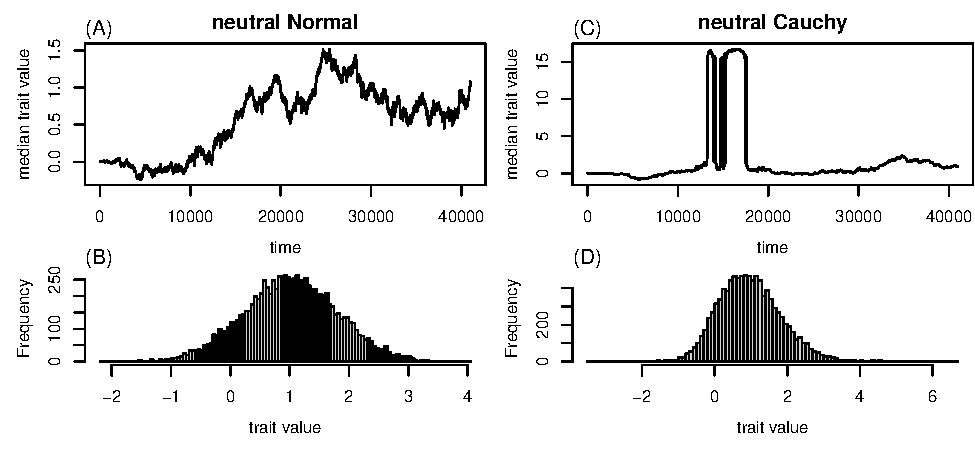
\includegraphics{sims/neutral_trait_traces}
    \end{center}
    \caption{
        Median trait values over time \textbf{(A and C)}
        and distributions of final trait values \textbf{(B and D)}
        in neutral simulations
        with Gaussian \textbf{(A and B)} and Cauchy \textbf{(C and D)}
        effect size distributions.
        Simulations were begun with no genetic variation,
        had populations of size $N=1000$,
        a genome of length $L=10^8$ bp and mutation rate of $\mu=10^{-9}$ per bp per generation;
        the effect size distributions were
        Normal with mean 0 and standard deviation $1/\sqrt{4NL\mu}$
        and Cauchy with center 0 and scale $1/(4NL\mu)$, respectively.
        \label{fig:trait_distrns}
    }
\end{figure}

\begin{figure}
    \begin{center}
        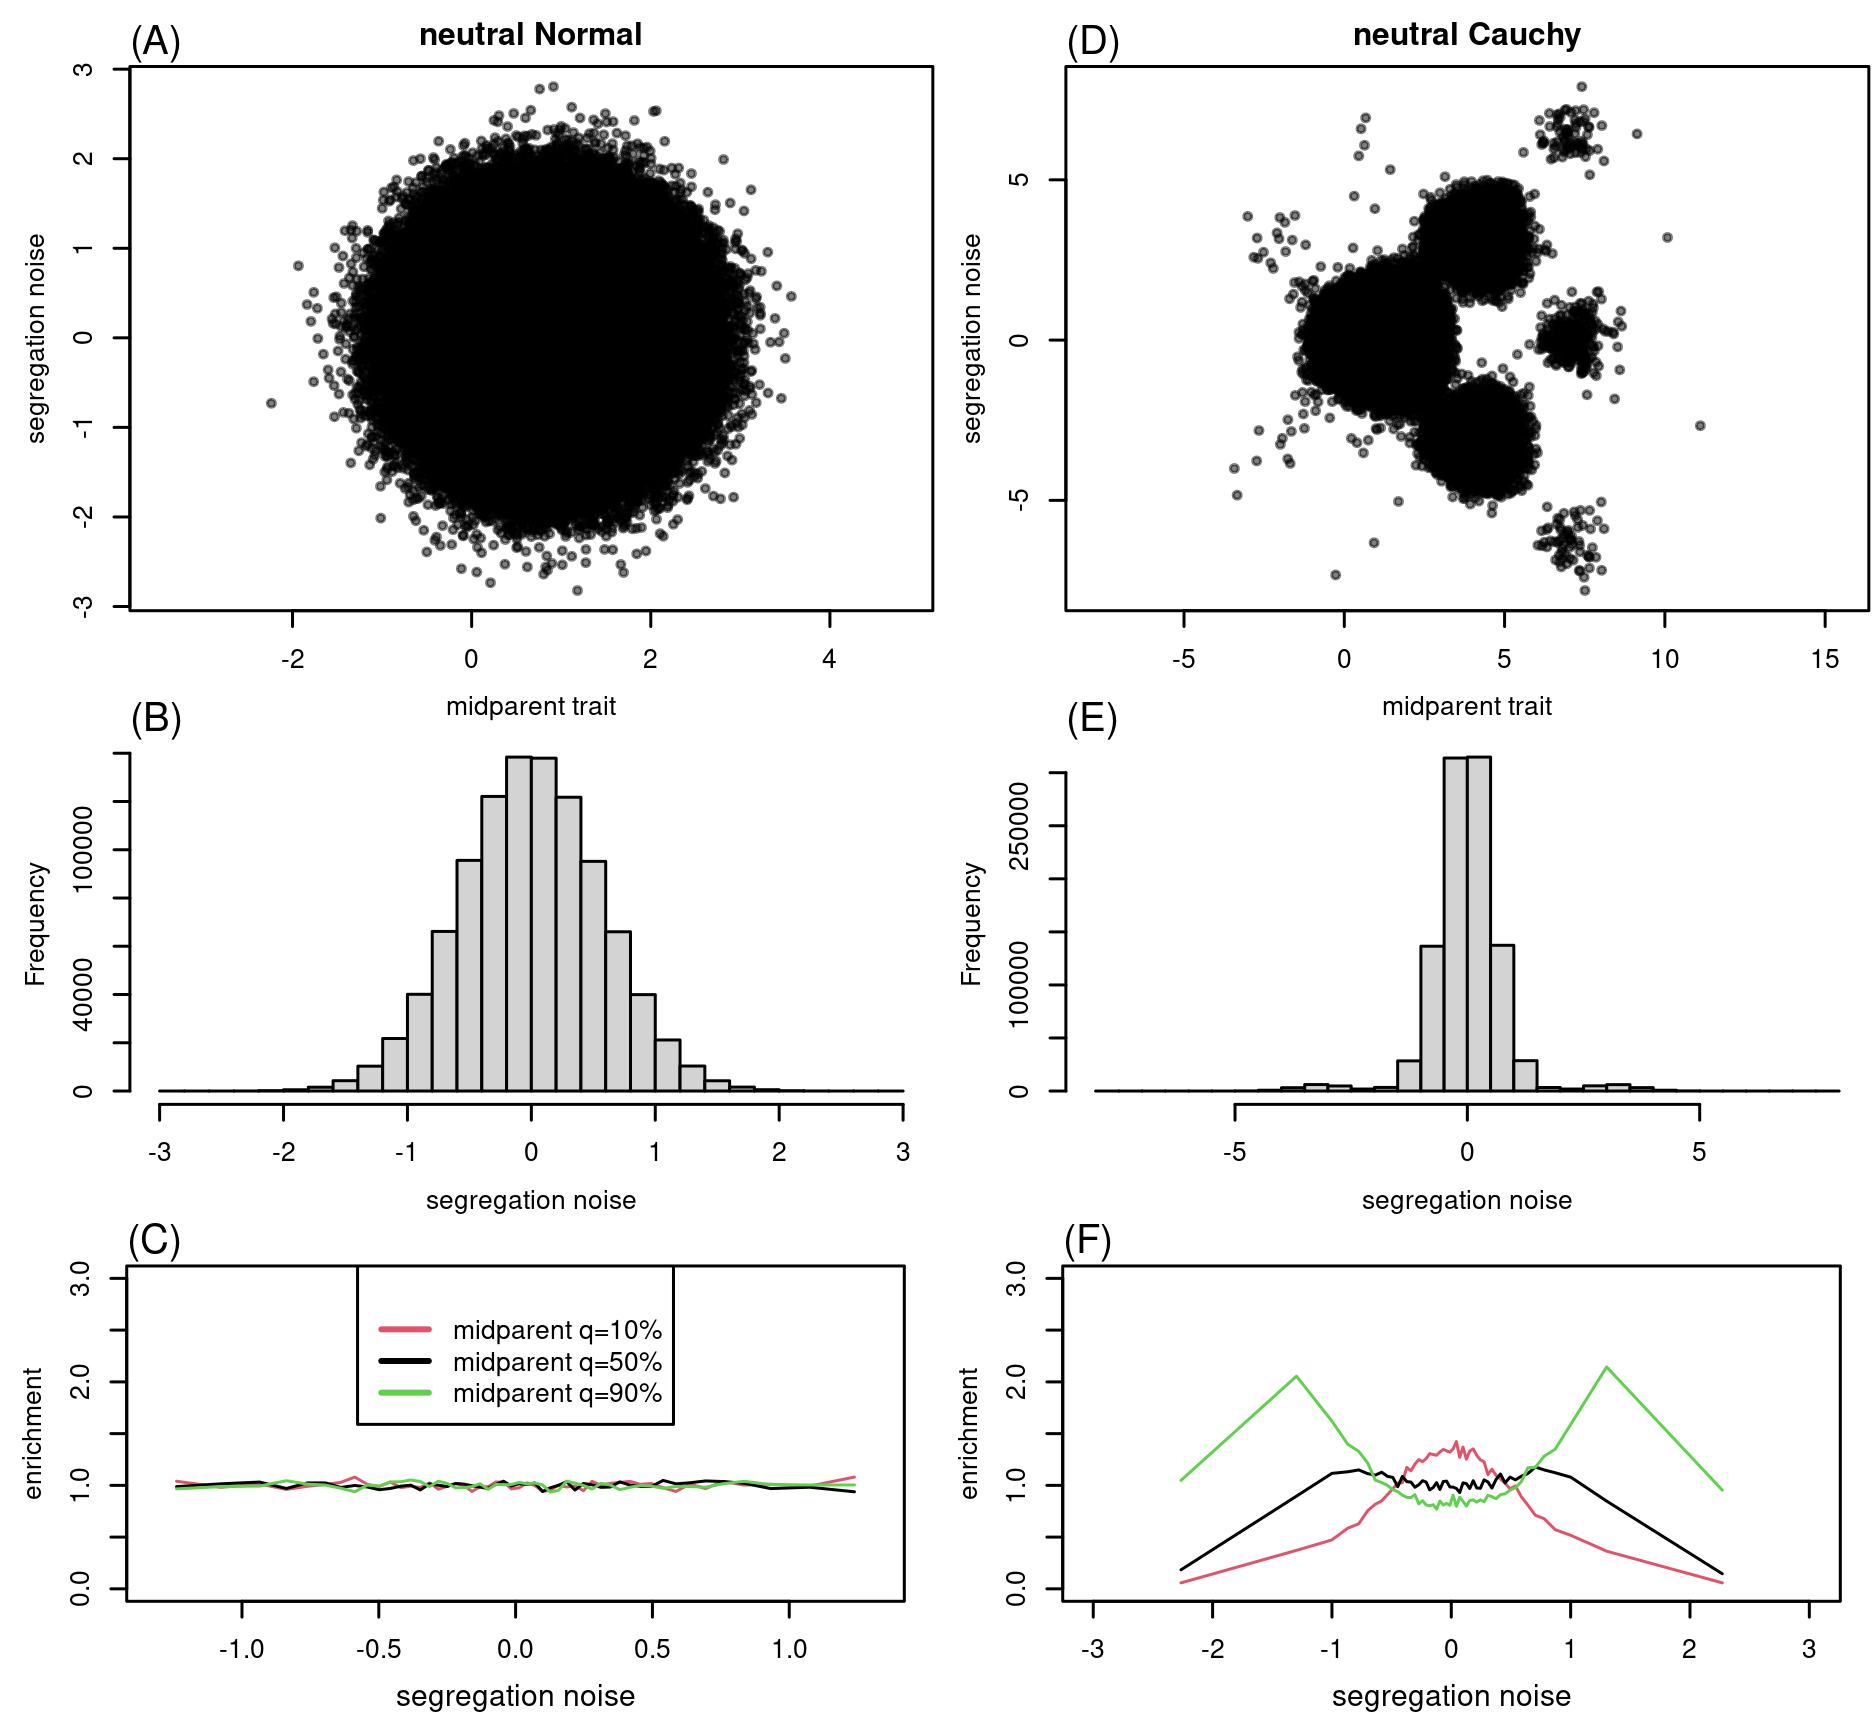
\includegraphics{sims/neutral_seg_noise}
    \end{center}
    \caption{
        The distribution of Mendelian sampling terms
        with Gaussian \textbf{(A-C)} and Cauchy \textbf{(D-F)} effect size distributions,
        from the same simulations shown in Figure~\ref{fig:trait_distrns},
        for all individuals born during the last 1,000 time units of the simulation.
        \textbf{(A,D)} Mendelian noise (offspring trait minus midparent) plotted against midparent.
        \textbf{(B,E)} Histograms of the Mendelian sampling term.
        \textbf{(B,E)} Enrichment in quantiles of the Mendelian sampling term conditional on midparent value.
        To compute the latter,
        let $q_0, q_2, q_4, \ldots, q_{98}, q_{100}$ divide the distribution of the Mendelian sampling term
        into 50 bins with roughly equal numbers in each (i.e., the quantiles),
        let $p_k(a,b)$ denote the proportion of the offspring of parents with midparent value
        is in $[a, b)$ whose Mendelian sampling term is in $[q_{k-1}, q_k)$,
        and let $p_k$ be the proportion of all offspring with Mendelian noise in $[q_{k-1}, q_k)$
        (so, $p_k \approx 0.02$).
        Then, each line shows $p_k(a,b)/p_k$
        plotted against the midpoint of the corresponding quantile bin $(q_{k-1},q_k)$,
        for $(a,b)$ chosen to span the three segments of 5\% of
        ``low'', ``medium'', and ``high'' midparents, i.e.:
        midparents between (red) the 7.5\% and 12.5\% quantiles,
        (black) the 47.5\% and 52.5\% quantiles, and
        (green) the 87.5\% and 92.5\% quantiles of midparent value.
        \label{fig:seg_noise}
    }
\end{figure}

We first consider the neutral case (i.e., with $\mu \equiv 1$).
As shown in Figure~\ref{fig:trait_distrns},
a simulation with a Cauchy effect size distribution, unsurprisingly,
has a distribution of trait values with more extreme values
and a rougher path of population median trait value over time
than does a simulation with a Gaussian effect size distribution.
Indeed, the sum of all effects along the path from the start of the simulation
to an arbitrary individual will approximate either Brownian motion (in the Gaussian case)
or a Cauchy process (in the Cauchy case).
Figure~\ref{fig:seg_noise} shows how the Mendelian sampling term
depends on midparent value.
In the Gaussian case, the Mendelian noise is Gaussian and independent of midparent value,
as shown by the horizontal lines at 1.0 in Figure~\ref{fig:seg_noise}C. 
On the other hand, in the Cauchy case we can see from either Figure~\ref{fig:seg_noise}D or F
that Mendelian noise depends strongly on midparent trait,
as we would expect in the presence of several large-effect alleles.

\begin{figure}
    \begin{center}
        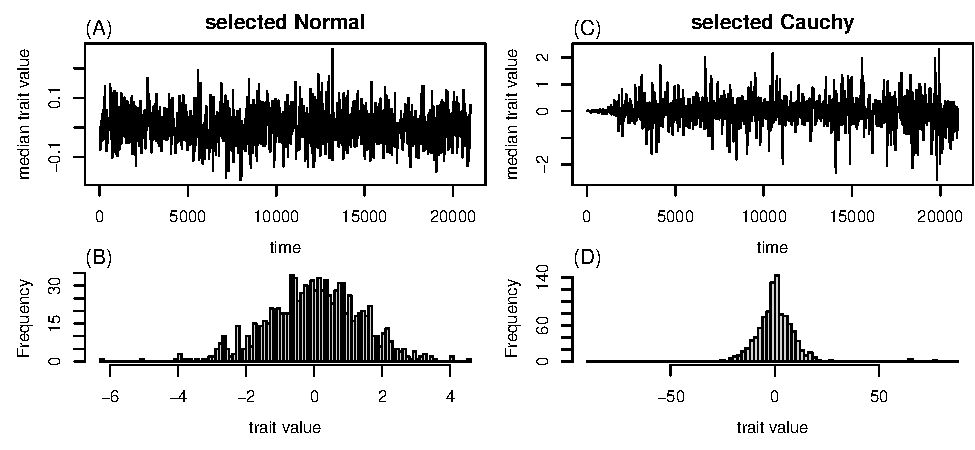
\includegraphics{sims/selected_trait_traces}
    \end{center}
    \caption{
        As in Figure~\ref{fig:trait_distrns},
        except under a model of stabilizing selection
        (see text for details,
        and note that the scale of the underlying mutations do not match
        neutral simulations, so distributions are not directly comparable
        to Figure~\ref{fig:trait_distrns}).
        \label{fig:sel_trait_distrns}
    }
\end{figure}

\begin{figure}
    \begin{center}
        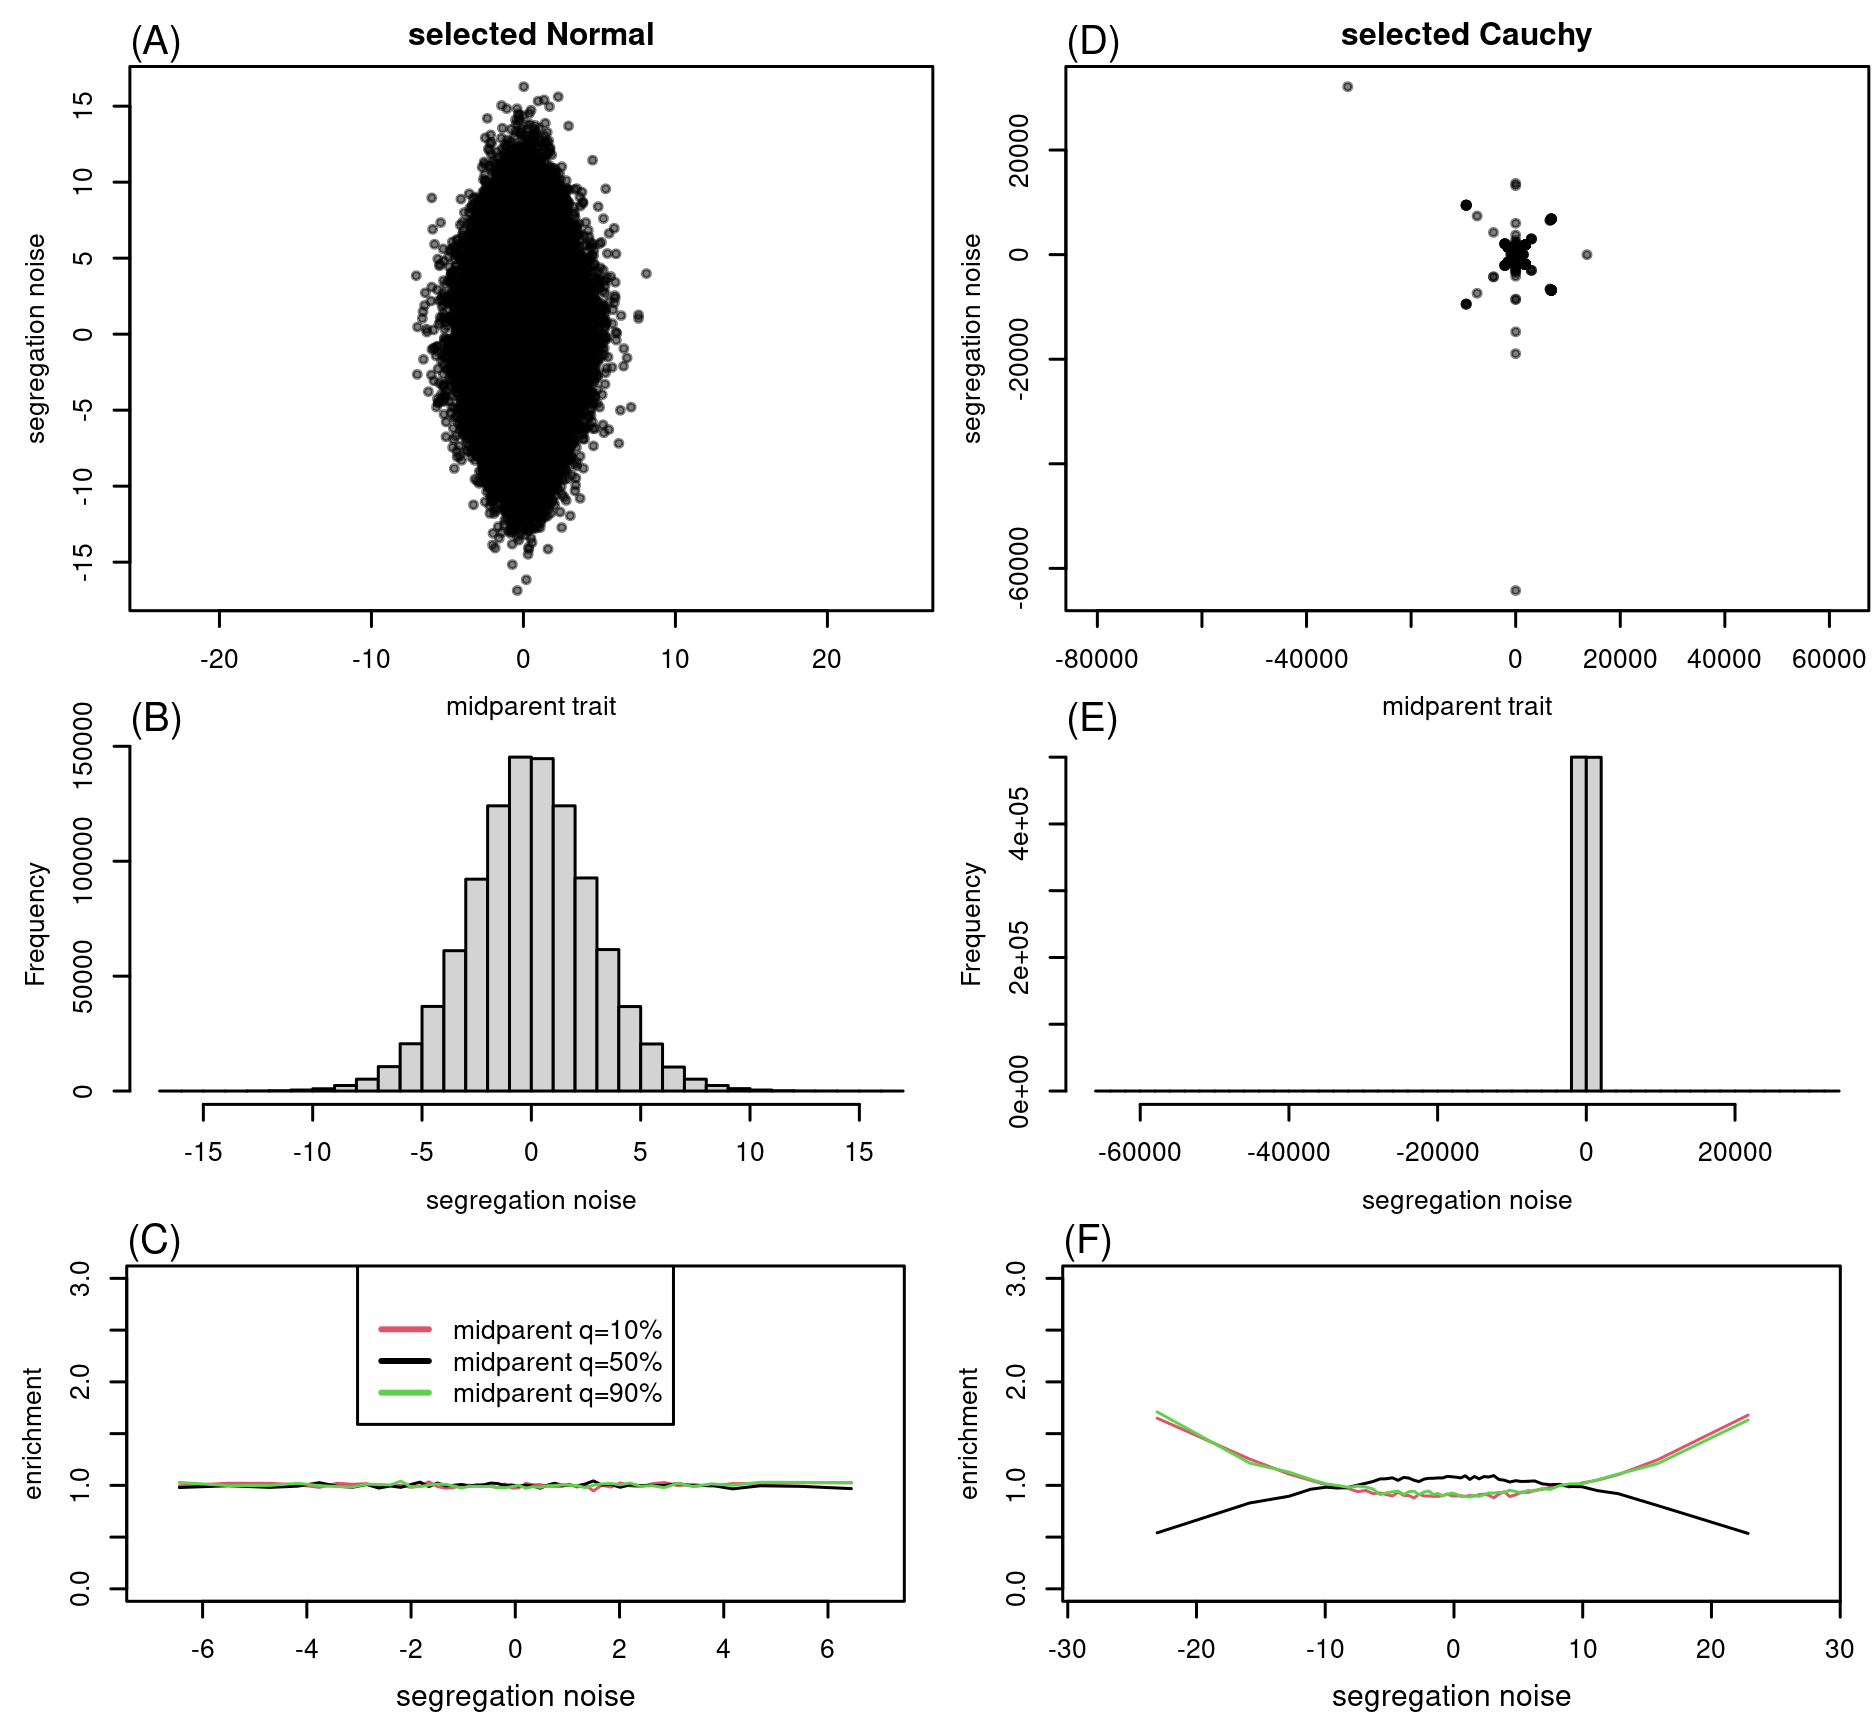
\includegraphics{sims/selected_seg_noise}
    \end{center}
    \caption{
        As in Figure~\ref{fig:seg_noise},
        except under a model of stabilizing selection (see text for details).
        \label{fig:sel_seg_noise}
    }
\end{figure}

We next compared two situations of stabilizing selection, motivated by the results
in Section~\ref{sec:stabilizing_selection}:
(1) the effect size distribution was Gaussian with mean zero and standard deviation 1.0
and $\mu(z) = e^{\alpha z^2}$; and
(2) the effect size distribution was Cauchy, centered at zero and with median absolute deviation $\delta - \gamma$
and $\mu(z) = (\delta/\gamma) (\gamma + z^2) / (\delta + z^2)$ with $\delta=0.5$ and $\gamma=0.2$.
Figures~\ref{fig:sel_trait_distrns} and~\ref{fig:sel_seg_noise}
show that the picture is largely unchanged by stabilizing selection
except that, unsurprisingly, the median trait no longer wanders unconstrained
(but still shows substantially larger fluctuations under the Cauchy model).

\begin{figure}
    \begin{center}
        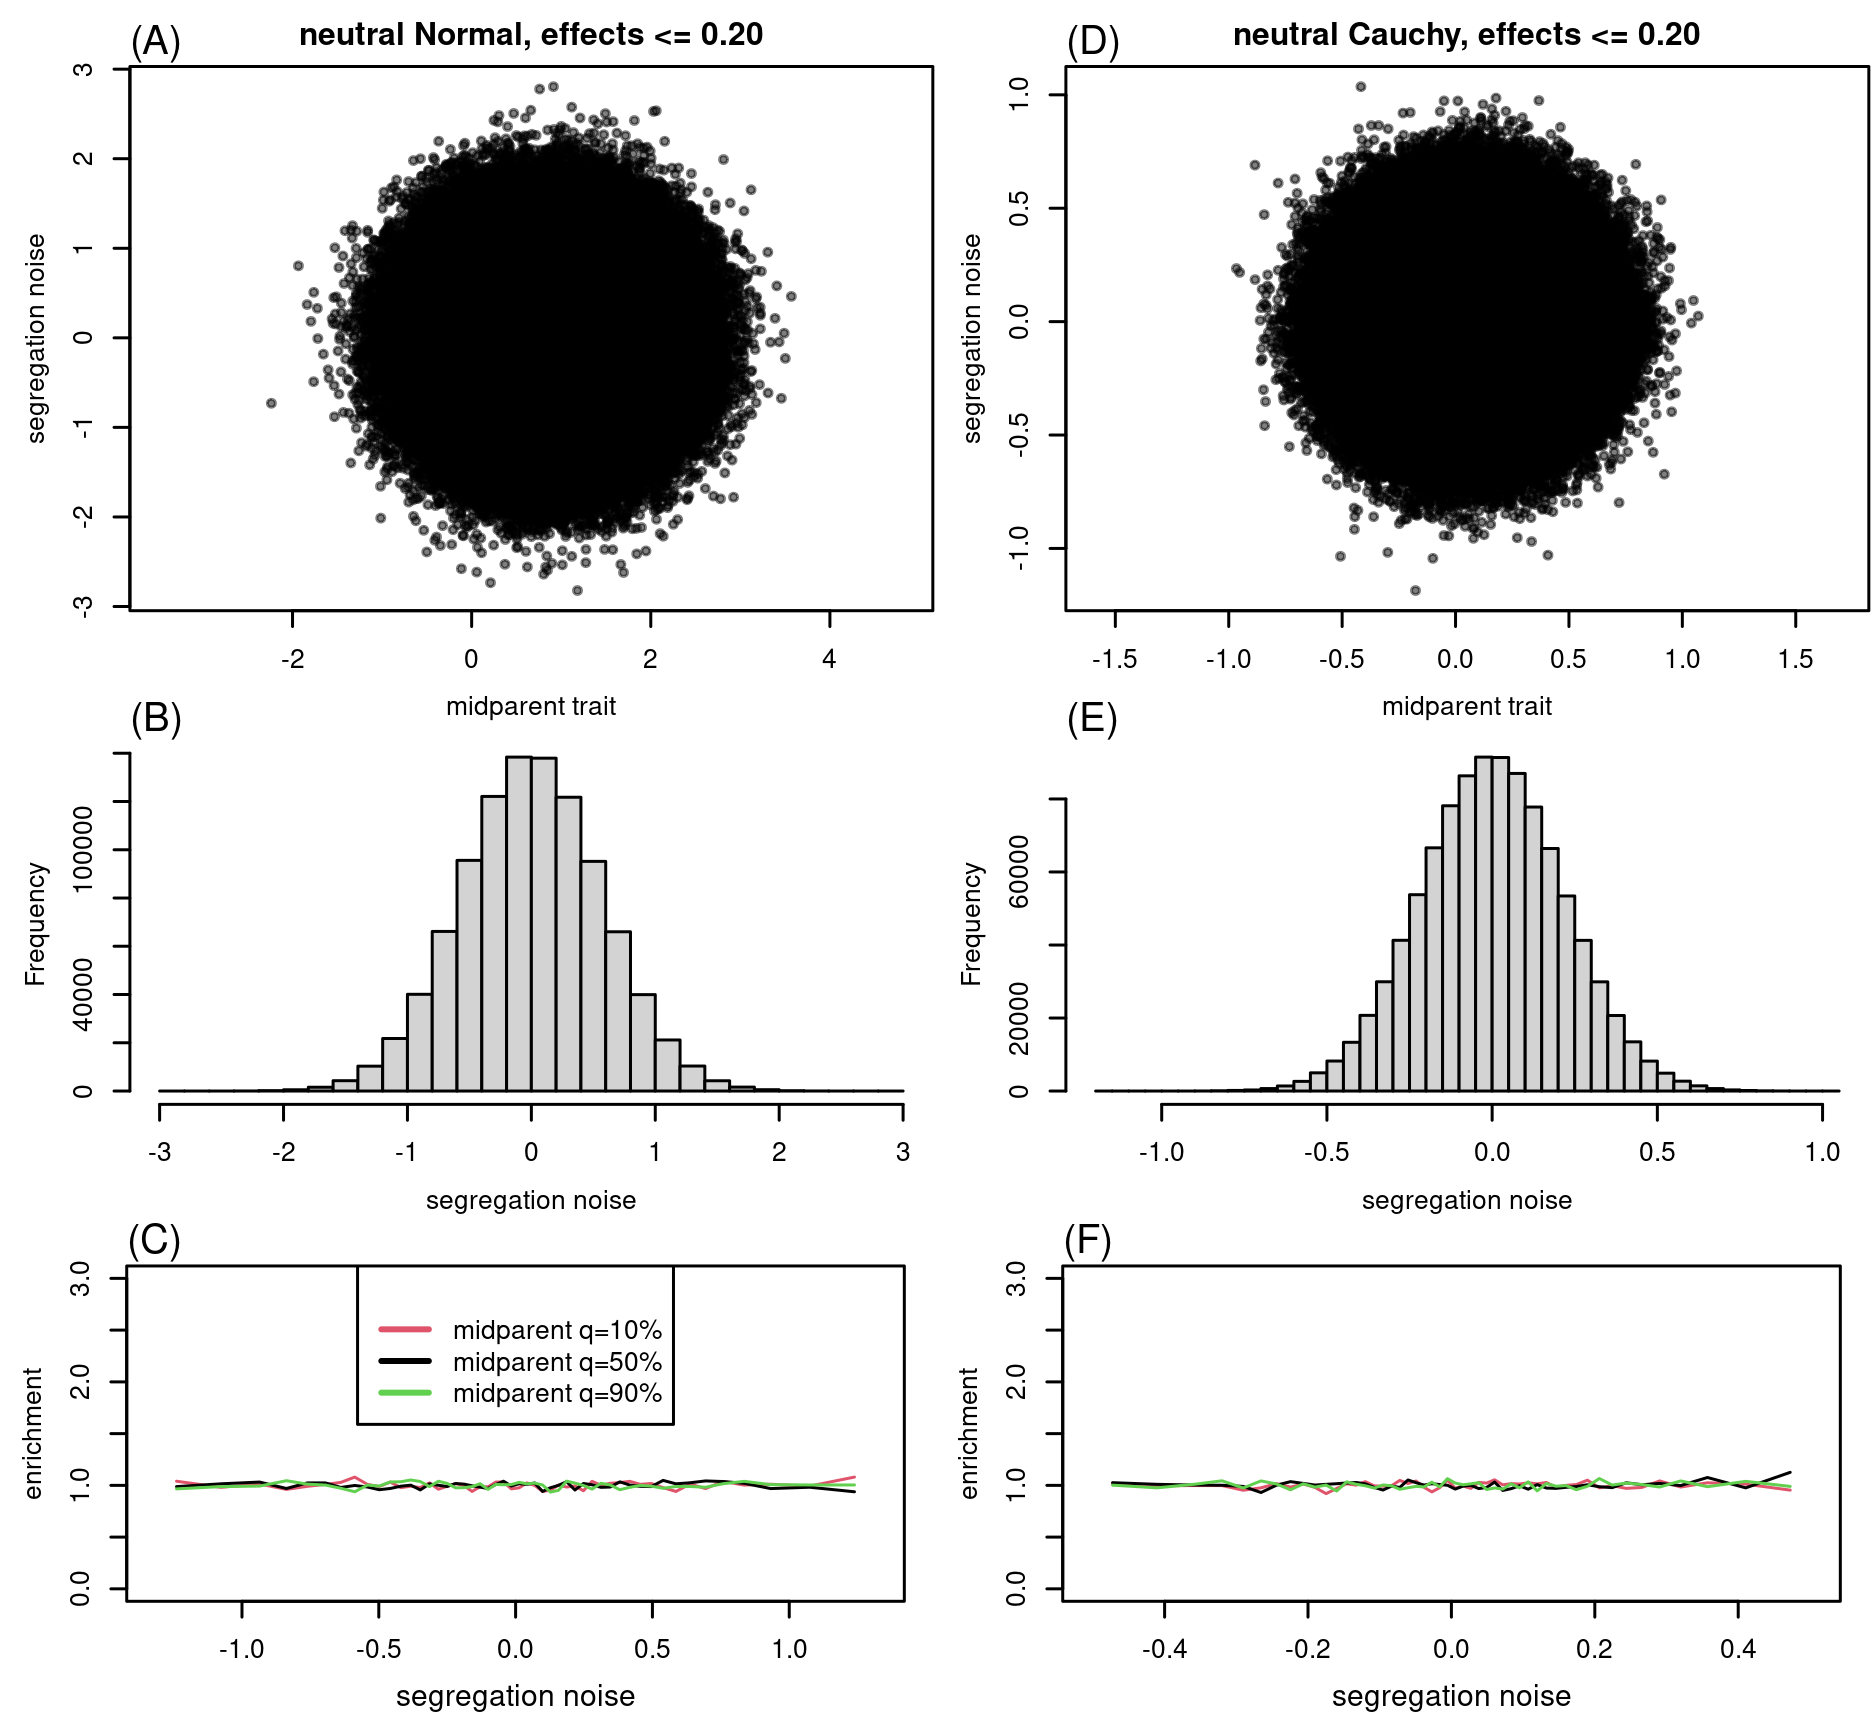
\includegraphics{sims/neutral_seg_noise_small}
    \end{center}
    \caption{
        As in Figure~\ref{fig:seg_noise},
        except computed using only mutations with absolute value effect size less than 0.2.
        The same quantities for the simulations of Figure~\ref{fig:sel_seg_noise}
        with stabilizing selection are shown in Figure~\ref{fig:sel_seg_noise_small}.
        \label{fig:seg_noise_small}
    }
\end{figure}


However,
the two models look much more similar when considering only alleles of small effect.
Figure~\ref{fig:seg_noise_small} shows that midparent values
and Mendelian sampling terms computed using only mutations with effect size less than 0.2
(excluding less than 1\% of mutations)
are quite close to independent.
The result does not depend strongly on the cutoff chosen,
and are similar even if less 0.1\% of mutations are excluded.

%%%%%%%%%%%%%%%%%%%%%%%
\section{Discussion}
    \revpoint{2}{11}

The infinitesimal model is a powerful and tractable model of trait inheritance,
but is polygenic to a fault,
excluding the possibility of loci of large effect
(that are often seen in practice).
In this paper,
we have looked at the possibility of using a broader range of central limit theorems
to extend the infinitesimal model to traits for which 
effect size distributions fall in the domain of attraction of the $\alpha$-stable distributions
(i.e., a larger proportion of variance
is explained by a smaller number of loci).
Indeed, we found evidence that this is true of many real traits,
although our relatively uncritical use of GWAS estimates makes this evidence suggestive at best.
Next, we show that in fact the infinitesimal model \emph{cannot} describe non-Gaussian distributions
\comment{XXX TODO}.
A recurring theme in the rest of the paper is
that just as the infinitesimal model is useful precisely because it ignores the genetic details,
it cannot apply once some genetic details are important
(i.e., there are loci of large effect).



A substantial challenge for the field is to develop tractable models of trait evolution
that include contributions of both ``large'' and ``small'' effect loci.
In practice, breeders have long embellished the ``animal model'' (essentially, the infinitesimal model)
to predict traits
by combining both effects of known large effect loci
and cumulative effects of many unknown loci as mediated by a relatedness matrix
\citep[e.g.,][]{fernando1989marker,teissier2018weighted,bernardo2014genomewide,rice2019evaluation}.
We can study any model with simulation,
but the way forwards to theoretical understanding seems murky.

Further analysis of the infinitesimal model with other noise distributions,
as we have begun here,
could be interesting,
e.g., to see how changing the distribution of the Mendelian sampling term
affects the rate of adaptive evolution,
levels of genetic load,
the rate of fixation,
and the strength of linked selection.
However,
we have seen that the assumption of independence in the infinitesimal model
implies a sort of ``blending inheritance''
for the large effect alleles,
and so such work must be accompanied by simulations
to see if the predictions are borne out under concrete models of genetic inheritance.
Another open question is whether there is some set of realistic assumptions
(perhaps involving epigenetic effects, pleiotropy, and/or environmental interactions with genetic effects)
which leads to these non-Gaussian infinitesimal models.
Finally, it may well be that there is a clever way to set up a trait-only model of evolution
that is both insensitive to the underlying genetics
and does not rely on the Gaussian central limit theorem.

Finally, we note that above we've most often used the Cauchy distribution
not because it seems most realistic
(indeed data suggests the $\alpha$-stable distribution with $\alpha=3/2$ might be better) \revpoint{2}{12}
but for mathematical convenience.

\subsection*{Selection and effect size distributions} \llabel{discussion_DFEs}
A substantial body of theoretical work has used various models and assumptions
to predict what distributions of effect sizes are expected based on biology.
In comparing to this work, there are several distinctions that are important to make.
For instance, selection makes the distribution of effect sizes identified by GWAS
different than the distribution of effect sizes of \emph{de novo} mutations,
and predictions are made about this relationship by \citet{simons2018population} % and \citet{simons2022simple}.
(under stabilizing selection)
and \citet{hayward2022polygenic}
(under adaptation to a new environment).
Our first question in this paper is orthogonal to this discussion:
\emph{given} the available genetic variation,
what model should we use to predict the short-term course of evolution?
As we saw in Section~\ref{sec:empirical},
the frequency-weighted effect size distribution (perhaps closer to that seen by GWAS)
is more relevant for this question than the \emph{de novo} effect size distribution.
In the latter part of this paper we look at long-term dynamics,
but with major differences:
most obviously, we only consider the distribution of the Mendelian noise term,
rather than the distribution of individual allelic effects.
These two are clearly related, but a more detailed analysis is beyond the scope of this paper.

\subsection*{Acknowledgements}
Thanks go to Nate Pope for useful discussion
and to Gregor Gorjanc for insight into modern uses
of the animal model and genomic selection. 
This project was started on a visit by TLP to the University of Oregon that was partially supported by the CNRS PEPS grant ``Jeunes Chercheuses et Jeunes Chercheurs''.

\bibliographystyle{plainnat}
\bibliography{refs}

\appendix
\setcounter{table}{0}
\renewcommand{\thetable}{S\arabic{table}}
\setcounter{figure}{0}
\renewcommand{\thefigure}{S\arabic{figure}}

\begin{figure}
    \begin{center}
    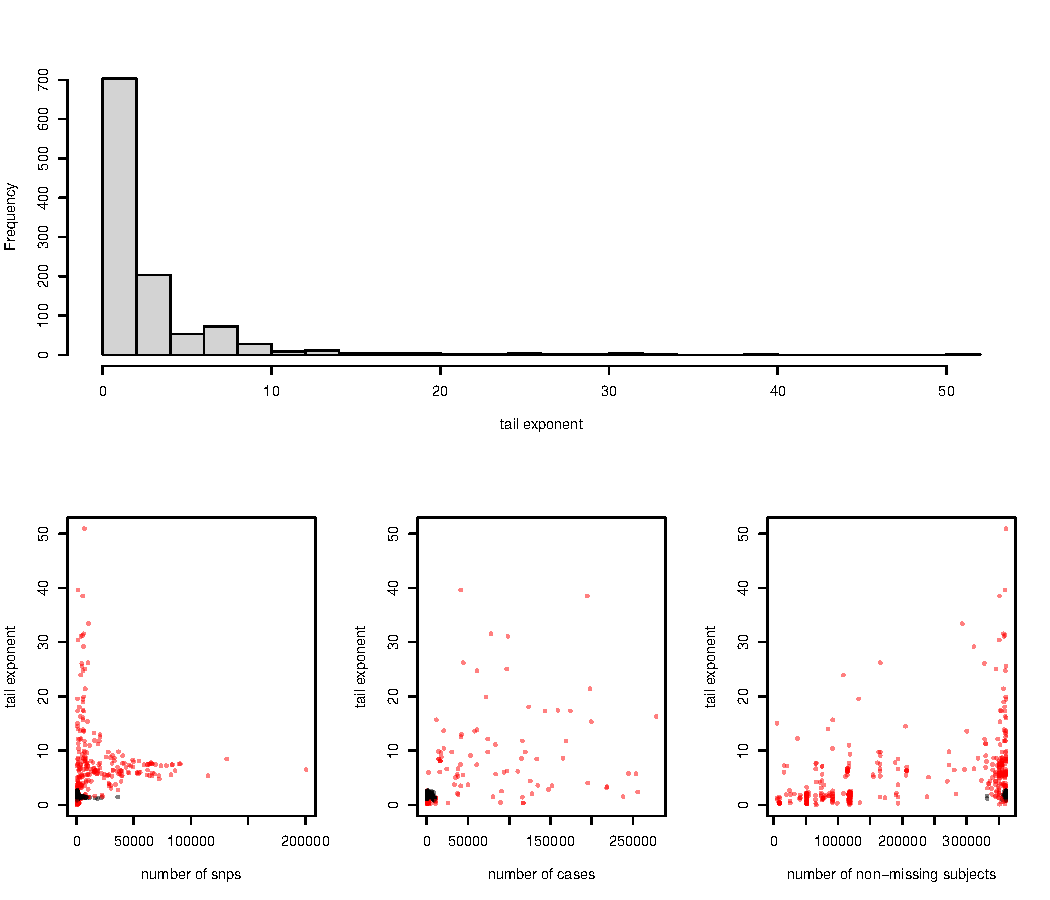
\includegraphics{snp_effects/unfiltered_results_10}
    \end{center}
    \caption{
        Estimated values of the tail exponent, $\alpha$,
        for 1108 illness-related binary phenotypes,
        including the 333 phenotypes removed in filtering,
        which are shown as red points in lower plots.
        \textbf{(A)} distribution of values; and plotted against
        \textbf{(B)} number of SNPs,
        \textbf{(C)} number of cases, and
        \textbf{(C)} number of non-missing subjects.
        \label{fig:unfiltered_hist}
    }
\end{figure}

\begin{figure}
    \begin{center}
        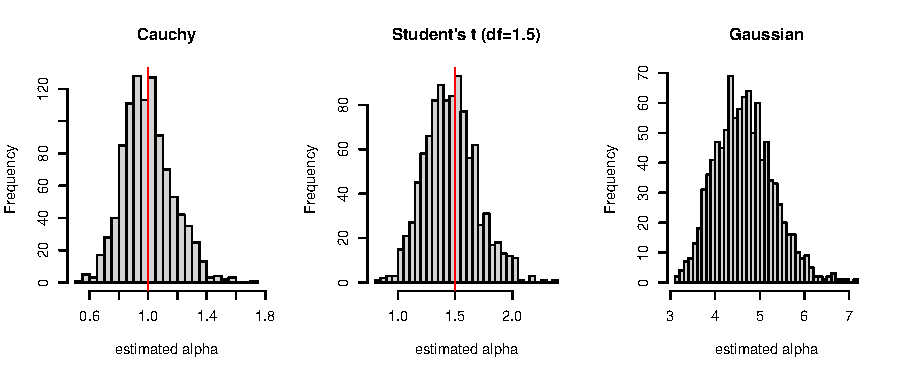
\includegraphics{snp_effects/power_demo}
    \end{center}
    \caption{
        Distributions of estimated tail exponents using the same estimator
        as in Figure~\ref{fig:exponent_hist},
        for 1000 independent draws from
        \textbf{(left)} the Cauchy distribution (true $\alpha=1$),
        \textbf{(center)} the Student's $t$ distribution with 1.5 degrees of freedom (true $\alpha=1.5$), and
        \textbf{(right)} the Gaussian distribution (true $\alpha$ is undefined,
        as the tail decays super-polynomially).
        Note that the typical number of SNPs per trait (shown in Figure~\ref{fig:exponent_hist})
        is around 1000.
        \label{fig:power}
    }
\end{figure}

\begin{figure}
    \begin{center}
        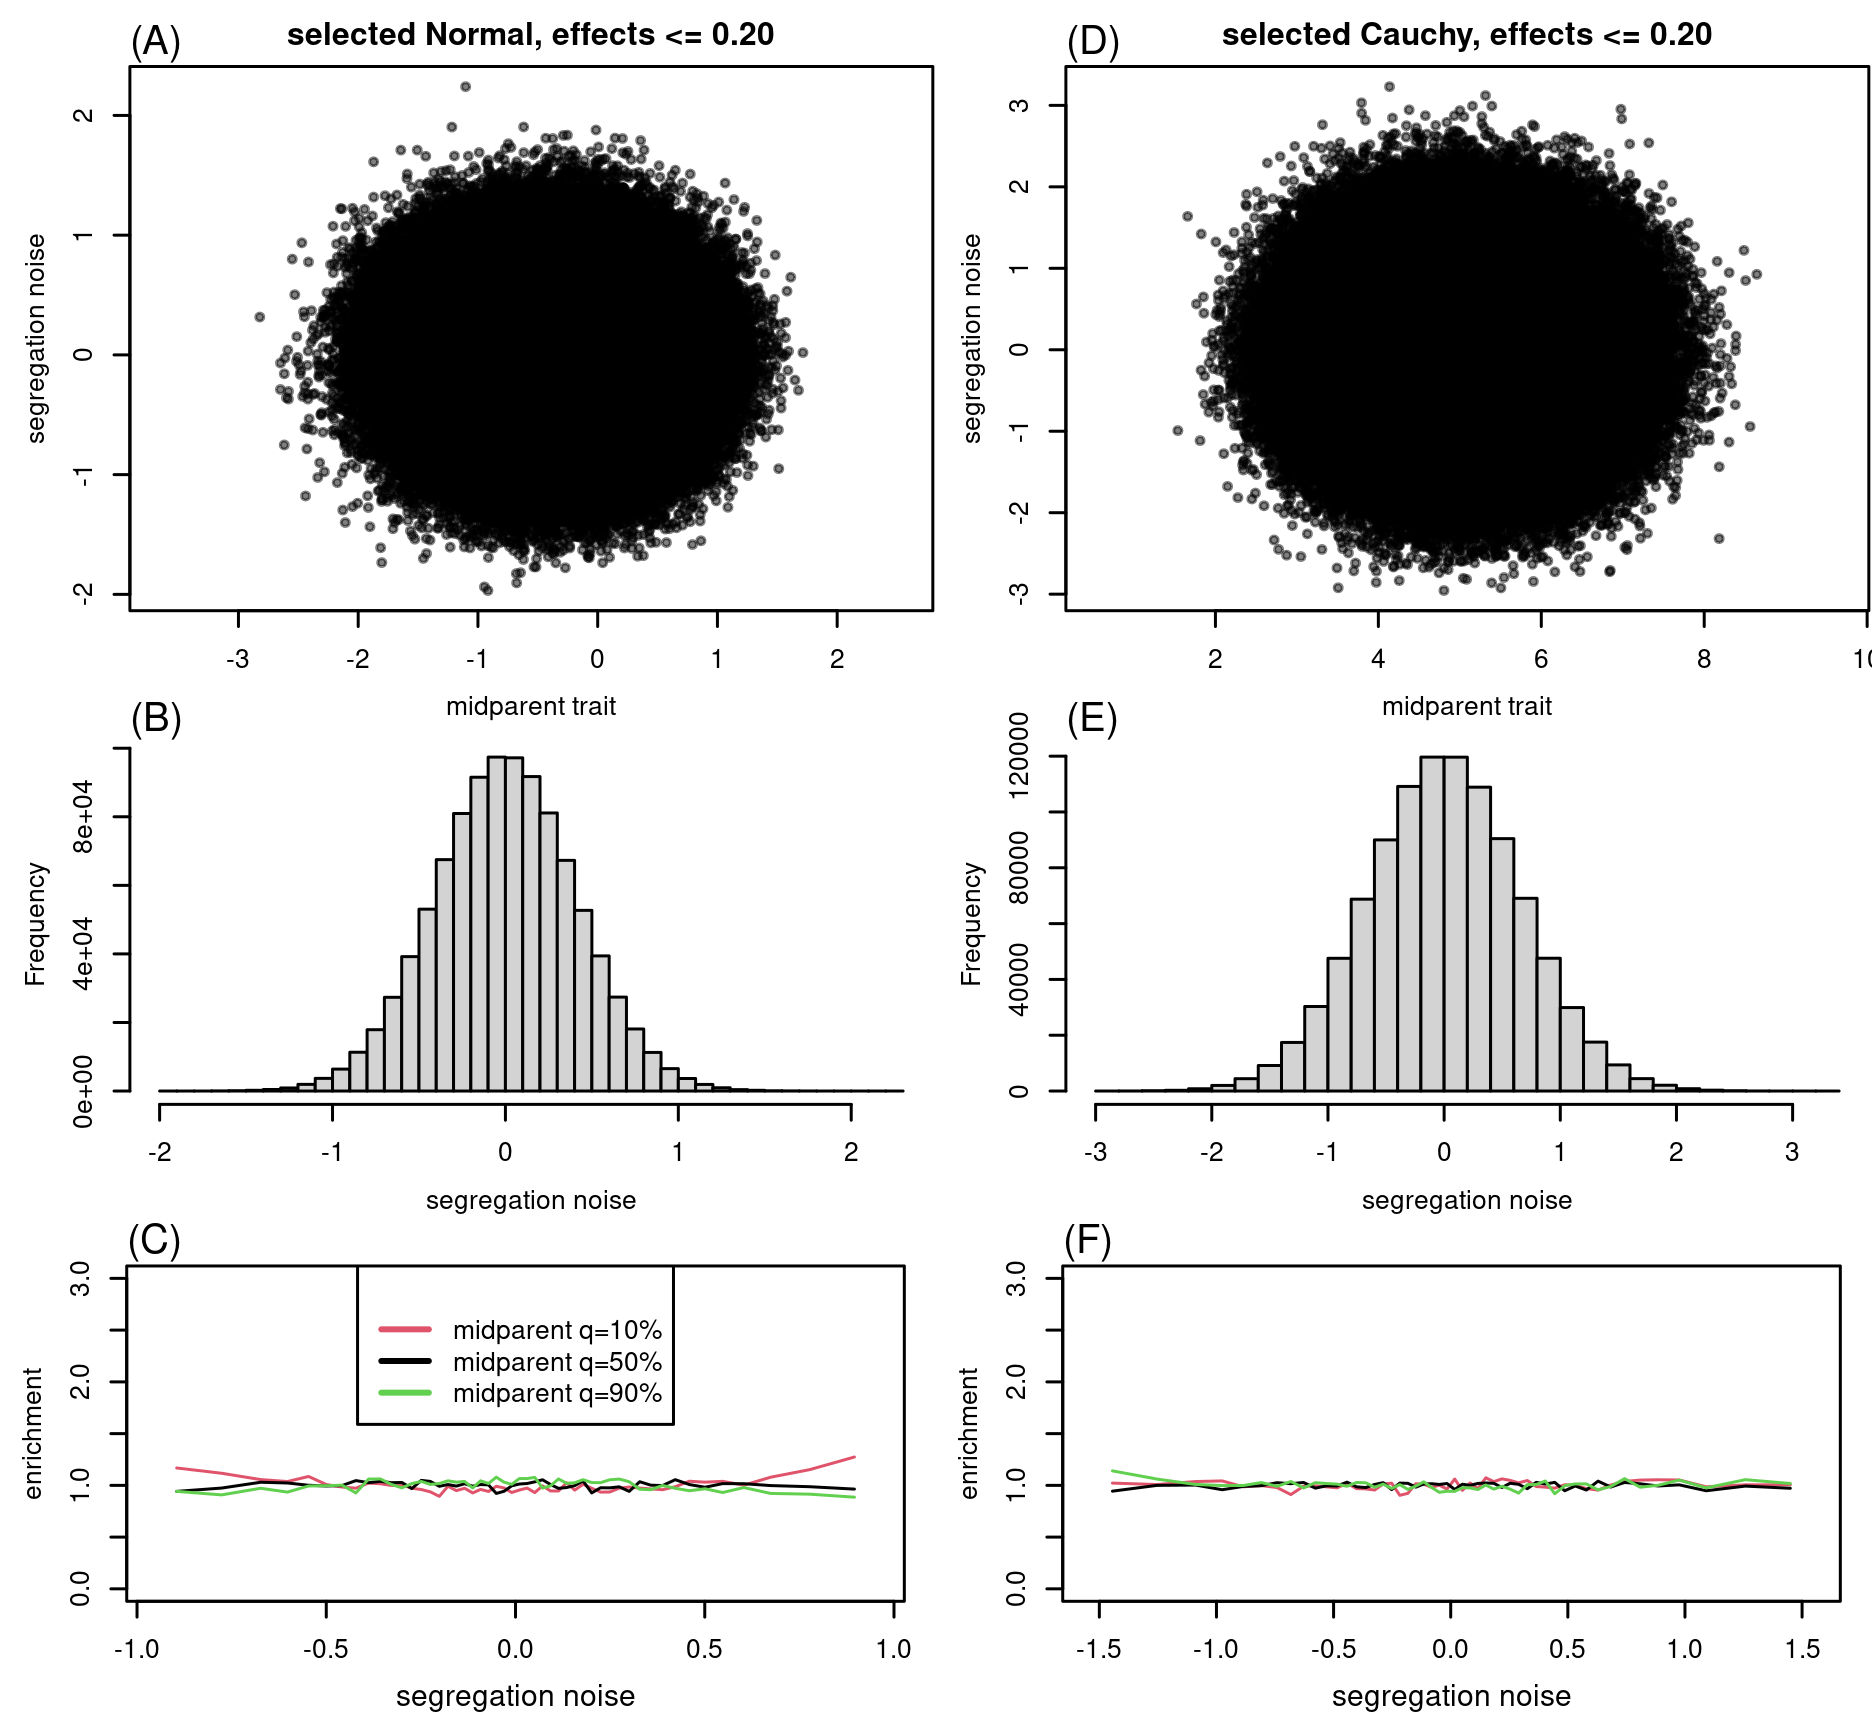
\includegraphics{sims/selected_seg_noise_small}
    \end{center}
    \caption{
        As in Figure~\ref{fig:seg_noise},
        except computed using only mutations with absolute value effect size less than 0.2.
        \label{fig:sel_seg_noise_small}
    }
\end{figure}

% reviews here if toggled above
% \ifsubmission\processdelayedfloats\fi

\includereviews


\end{document}
